% $Id: llcf-api.tex,v 1.24 2006/02/20 14:24:33 hartko Exp $

\documentclass[a4paper]{article}

\usepackage{german,umlaut}
\usepackage{geometry}
\usepackage{latexsym}
\usepackage{verbatim}
\usepackage{color}		% Need the color package
\usepackage{epsfig}
\geometry{body = {6in, 9in}}
\sloppy


\parindent0pt

%\includeonly{socket-api}

% $Id: llcftexdefs.tex,v 1.7 2005/06/30 16:52:23 hartko Exp $

\newcommand {\LL}{\textbf{\mbox{LLCF}}}
\newcommand {\LLCF}{\emph{\mbox{Low Level CAN Framework}}}
\newcommand {\BC}{\textbf{\mbox{BCM}}}
\newcommand {\BCM}{\emph{\mbox{Broadcast-Manager}}}

\newenvironment{code}{\begingroup\quote\renewcommand{\baselinestretch}{0.8}\verbatim}{\endverbatim\endquote\endgroup}

\def\man#1#2{\textsf{#1(#2)}}


\begin{document}

\begin{figure}[htbp]
\begin{center}

\psfig{file=llcf-2003-10-22-final.eps}
\end{center}
\end{figure}

\begin{center}
%{\Huge Low Level CAN Framework}\\
%\vspace{0.4cm}
{\LARGE Application Programmers Interface}
\end{center}

\vspace{0.7cm}
\centerline{\large Version 1.0.0}
\vspace{0.7cm}
\centerline{\large 2006-02-20}
\vspace{0.7cm}

\newpage

\tableofcontents

% $Id: intro.tex,v 1.3 2005/07/05 08:05:42 hartko Exp $

\newpage
\section{Einleitung}
\label{intro}

Im Rahmen verschiedener Projekte wurde in der Konzernforschung der
Volkswagen AG
ein so genanntes \LLCF\ (\LL) entwickelt, das den einfachen Zugriff
auf die Kommunikationsschichten des {\it Controller Area Network}
(CAN) f�r Anwendungen erlaubt.  Das \LLCF\ sollte dabei m�glichst
modular konzipiert werden, um eine m�glichst gro�e
Wiederverwendbarkeit in weiteren Projekten zu erreichen.\\

Wesentliche Komponenten des \LL\ sind die Netzwerk(!)-Treiber f�r die
verschiedenen CAN-Controller und die dar�berliegenden Protokolle wie
TP1.6,
TP2.0, MCNet, ISO-TP, etc.  Diese Komponenten sind im Linux-Kernel
implementiert und  werden �ber die standardisierte
Socket-Schnittstelle angesprochen. Das Ziel dieses Konzeptes liegt
darin, die Kommunikation �ber 
den CAN-Bus soweit wie m�glich an die Benutzung gew�hnlicher
TCP/IP-Sockets anzupassen.  Dies gelingt jedoch nur zum Teil, da der
CAN-Bus eine Reihe von Unterschieden zur Kommunikation mit TCP/IP und
Ethernet aufweist:

\begin{itemize}
\item CAN kennt keine Ger�te-Adressen wie die MAC-Adressen beim Ethernet.
  Das CAN-Frame enth�lt eine CAN-ID, die durch die �bliche
  Zuordnung von zu sendenen CAN-IDs zu realen Endger�ten am ehesten einer
  Absender-Adresse entspricht.  Weil alle Nachrichten
  Broadcast-Nachrichten sind, ist es auch nicht m�glich, eine
  CAN-Nachricht nur an ein Ger�t zu senden. Ger�te am CAN-Bus k�nnen
  empfangene Nachrichten also nicht nach Zieladressen, sondern nur
  nach der CAN-ID 'Absenderadresse' filtern. CAN-Frames k�nnen daher
  nicht - wie beim Ethernet - explizit an ein bestimmtes Zielger�t
  gerichtet werden.  

\item Es gibt keinen Network Layer und damit auch keine
  Network-Layer-Adressen wie IP-Adressen. Folglich gibt es auch kein
  Routing (z.B. �ber verschiedene Netzwerk-Interfaces), wie es mit
  IP-Adressen m�glich ist. 
\end{itemize}

\begin{figure}[htbp]
\begin{center}

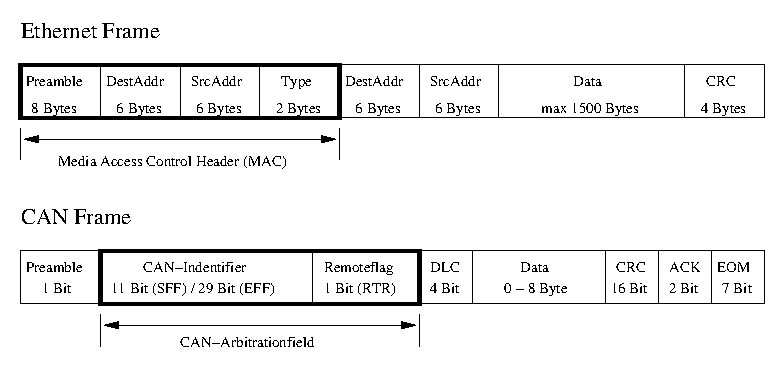
\psfig{file=frame_types.eps}

\caption{Unterschiedliche Adressierungen bei Ethernet /  CAN}
\label{figure:frame_types}
\end{center}
\end{figure}

Diese Unterschiede f�hren dazu, dass die Struktur
\verb|struct sockaddr_can| sich nicht ganz analog zu der bekannten
\verb|struct sockaddr_in| f�r die TCP/IP-Protokollfamilie verh�lt.
Der Ablauf eines Verbindungsaufbaus und die Benutzung ge�ffneter
Sockets zum Datenaustausch sind jedoch stark an TCP/IP angelehnt.

Neben diesem Dokument sind daher auch die Manual Pages
\man{socket}{2}, \man{bind}{2}, \man{listen}{2},
\man{accept}{2}, \man{connect}{2}, \man{read}{2},
\man{write}{2}, \man{recv}{2}, \man{recvfrom}{2},
\man{recvmsg}{2}, \man{send}{2}, \man{sendto}{2},
\man{sendmsg}{2}, \man{socket}{7}, \man{packet}{7} eines
aktuellen Linux-Systems f�r das \LL\ relevant.  Au�erdem bieten die
Manual Pages \man{ip}{7}, \man{udp}{7} und \man{tcp}{7} einen
Einblick in Grundlagen, auf denen auch das \LL\ basiert.

\newpage
Das \LLCF\ ist neben den bekannten Protokollen, wie z.B. den
Protokollen der Internetprotokollfamilie PF\_INET im Linux-Kernel
integriert. Dazu wurde eine neue Protokollfamilie PF\_CAN
eingef�hrt. Durch die Realisierung der verschiedenen CAN-Protokolle
als Kernelmodule, k�nnen zeitliche Randbedingungen im Kernel-Kontext
eingehalten werden, die auf der Anwenderschicht in dieser Form nicht
realisierbar w�ren. F�r verschiedene Anwendungen (was zu mehreren
Socket-Instanzen f�hrt) kommt immer derselbe Code zur Ausf�hrung.\\ 

\begin{figure}[htbp]
\begin{center}

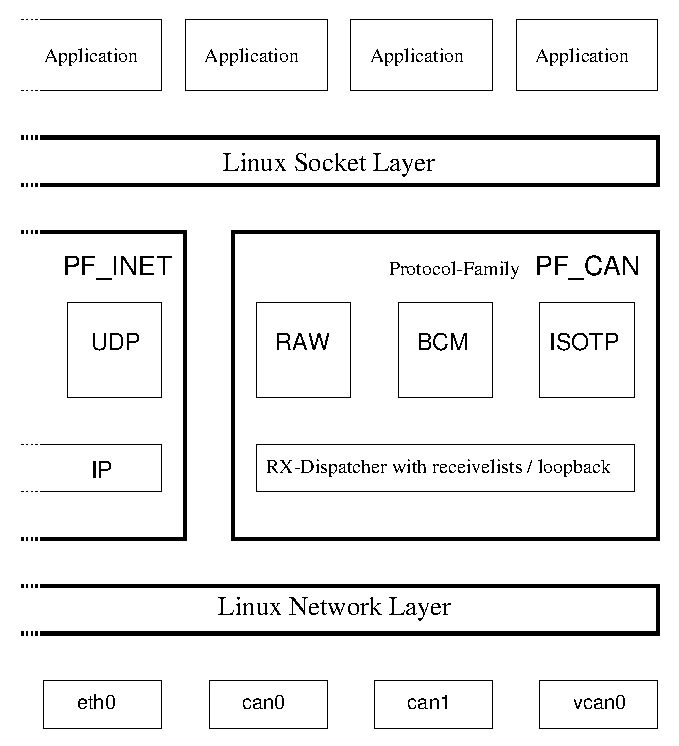
\psfig{file=llcf_overview.eps}

\caption{Das \LL\ im Linux-Kernel}
\label{figure:llcf_overview}
\end{center}
\end{figure}

Das \LL\ stellt f�r die verschiedenen Transportprotokolle und einen
so genannten \BCM\ (\BC) eine Reihe verschiedener Socket-Typen
zur Verf�gung.  Au�erdem ist ein RAW-Socket vorgesehen, der den
direkten Zugriff auf den CAN-Bus ohne dazwischenliegende
Protokollschichten erlaubt.

\newpage
Eine Besonderheit stellt der so genannte RX-Dispatcher des \LL\
dar. Durch die Art der Adressierung der CAN-Frames kann es
mehrere 'Interessenten' an einer empfangenen CAN-ID geben. Durch die
\LL-Funktionen rx\_register() und rx\_unregister() k�nnen sich die
Protokollmodule beim \LL-Kernmodul f�r ein oder mehrere CAN-IDs von
definierten CAN-Netzwerkger�ten registrieren, die ihnen beim Empfang
automatisch zugestellt werden. Das \LL-Kernmodul sorgt beim Senden auf
den CAN-Bus auch f�r ein lokales Echo ('local loopback') der zu
versendenden CAN-Frames, damit f�r alle Applikationen auf einem System
die gleichen Informationen verf�gbar sind.


\begin{figure}[htbp]
\begin{center}

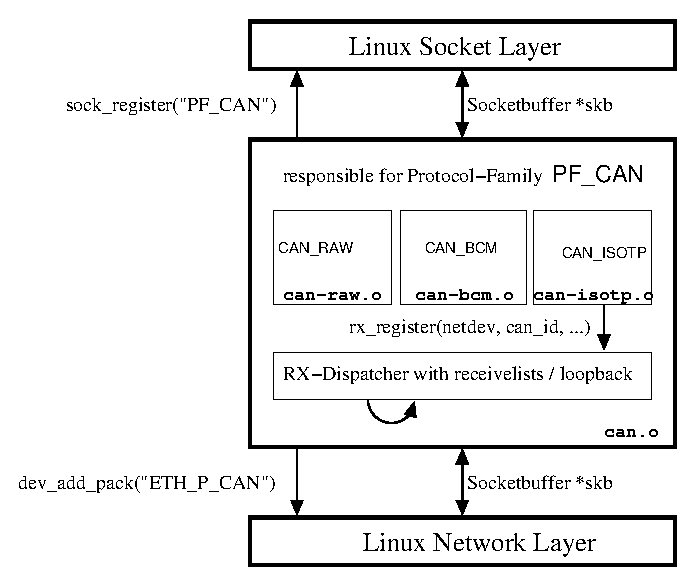
\psfig{file=llcf_module.eps}

\caption{Das \LL-Kernmodul im Linux-Kernel}
\label{figure:llcf_module}
\end{center}
\end{figure}

F�r die Anbindung der CAN-Netzwerktreiber wurde ein neuer
'Ethernet-Protokoll-Typ' ETH\_P\_CAN eingef�hrt, der die Durchleitung
der empfangenen CAN-Frames durch die Linux-Netzwerkschicht
sicherstellt. Das \LL-Kernmodul meldet sich dazu als Empf�nger von
ETH\_P\_CAN-'Ethernetframes' beim Kernel an.\\

Durch die konsequente Realisierung der Anbindung des CAN-Busses mit
Schnittstellen aus der etablierten Standard-Informationstechnologie
er�ffnen sich f�r den Anwender (Programmierer) alle M�glichkeiten, die
sich auch sonst bei der Verwendung von Sockets zur Kommunikation
ergeben. D.h. es k�nnen beliebig viele Sockets (auch verschiedener
Socket-Typen auf verschiedenen CAN-Bussen) von einer oder mehreren
Applikationen gleichzeitig ge�ffnet werden. Bei der Kommunikation auf
verschiedenen Sockets kann beispielsweise mit \man{select}{2} auf
Daten aus den einzelnen asynchronen Kommunikationskan�len
ressourcenschonend gewartet werden. 



% $Id: legal.tex,v 1.5 2006/02/08 14:38:21 hartko Exp $

\newpage
\section{Rechtliche Hinweise}
\label{legal}

Volkswagen geht davon aus, dass diese rechtlichen Hinweise vom
Anwender gelesen, verstanden und akzeptiert worden sind.

\medskip
Im Quellcode des \LLCF\ findet man folgenden Hinweis:

\begin{code}
/*
 * Copyright (c) 2002-2005 Volkswagen Group Electronic Research
 * All rights reserved.
 *
 * Redistribution and use in source and binary forms, with or without
 * modification, are permitted provided that the following conditions
 * are met:
 * 1. Redistributions of source code must retain the above copyright
 *    notice, this list of conditions, the following disclaimer and
 *    the referenced file 'COPYING'.
 * 2. Redistributions in binary form must reproduce the above copyright
 *    notice, this list of conditions and the following disclaimer in the
 *    documentation and/or other materials provided with the distribution.
 * 3. Neither the name of Volkswagen nor the names of its contributors
 *    may be used to endorse or promote products derived from this software
 *    without specific prior written permission.
 *
 * Alternatively, provided that this notice is retained in full, this
 * software may be distributed under the terms of the GNU General
 * Public License ("GPL") version 2 as distributed in the 'COPYING'
 * file from the main directory of the linux kernel source.
 *
 * The provided data structures and external interfaces from this code
 * are not restricted to be used by modules with a GPL compatible license.
 *
 * THIS SOFTWARE IS PROVIDED BY THE COPYRIGHT HOLDERS AND CONTRIBUTORS
 * "AS IS" AND ANY EXPRESS OR IMPLIED WARRANTIES, INCLUDING, BUT NOT
 * LIMITED TO, THE IMPLIED WARRANTIES OF MERCHANTABILITY AND FITNESS FOR
 * A PARTICULAR PURPOSE ARE DISCLAIMED. IN NO EVENT SHALL THE COPYRIGHT
 * OWNER OR CONTRIBUTORS BE LIABLE FOR ANY DIRECT, INDIRECT, INCIDENTAL,
 * SPECIAL, EXEMPLARY, OR CONSEQUENTIAL DAMAGES (INCLUDING, BUT NOT
 * LIMITED TO, PROCUREMENT OF SUBSTITUTE GOODS OR SERVICES; LOSS OF USE,
 * DATA, OR PROFITS; OR BUSINESS INTERRUPTION) HOWEVER CAUSED AND ON ANY
 * THEORY OF LIABILITY, WHETHER IN CONTRACT, STRICT LIABILITY, OR TORT
 * (INCLUDING NEGLIGENCE OR OTHERWISE) ARISING IN ANY WAY OUT OF THE USE
 * OF THIS SOFTWARE, EVEN IF ADVISED OF THE POSSIBILITY OF SUCH
 * DAMAGE.
 *
 * Send feedback to <llcf@volkswagen.de>
 *
 */
\end{code}


\subsection{Erweiterter Haftungsausschluss}

Im Geltungsbereich der deutschen Rechtsprechung besteht auch bei der
kostenlosen �berlassung bei grob fahrl�ssigen oder 
vors�tzlich verschwiegenen M�ngeln die M�glichkeit, den Urheber f�r
entstandene (Folge-)Sch�den haftbar machen zu k�nnen.\\ 

Wenngleich die Autoren bem�ht sind, eine fehlerfreie Software zur
 Verf�gung zu stellen, lassen sich Fehler nicht generell
 ausschlie�en. Aus
 diesem Grunde erkl�rt sich der Anwender mit dem Einsatz des  
\LLCF\ damit einverstanden, den Haftungsausschluss gegen�ber den
Autoren und der Volkswagen AG {\bf uneingeschr�nkt} anzuerkennen und
auf jedwede rechtlichen M�glichkeiten/Forderungen beim Auftreten von
M�ngeln/Sch�den/Folgesch�den durch den Einsatz des \LL\ zu
verzichten.

\subsection{Logo}

Das Logo des \LLCF\ ( '/dev/$<$ beetle $>$' ) ist als zusammengesetzte
Bildmarke Eigentum der Volkswagen AG. Es symbolisiert die Integration
des Fahrzeugs in eine Umgebung der Standard-Informationstechnologie.

\subsection{Linux Module License}

Teile der vollst�ndigen \LL-Distribution unterliegen nicht der GNU Public
License sondern sind propriet�rer Code der Volkswagen
AG. Richtigerweise ist dieses auch im Quellcode der einzelnen
Kernelmodule mit dem Makro {\mbox{\bf MODULE\_LICENSE(\grqq Volkswagen
Group closed source\grqq)}} markiert. Beim Laden der \LL-Module in den
Kernel kann daher beispielsweise folgende Fehlermeldung auftreten:

\begin{code}
Warning: loading can-tp20.o will taint the kernel: Volkswagen Group closed source
See http://www.tux.org/lkml/#export-tainted for information about tainted modules
Module tainted loaded, with warnings
\end{code}

Dieses ist eine Warnung, dass das geladene Modul nicht unter der GNU
Public License steht, was die Funktionsf�higkeit des \LLCF\ jedoch nicht
beeinflusst. Typischerweise werden jedoch Anfragen zu Fehlermeldungen,
die von 'verschmutzten' tainted-Kernels erzeugt wurden, im Allgemeinen
von der Linux-Community nicht kommentiert / beantwortet.\\ 

Module, die unter der GNU Public License stehen, enthalten das Makro
{\mbox{\bf MODULE\_LICENSE(\grqq GPL\grqq)}}.

\subsection{Transportprotokolle}

Die in der vollst�ndigen \LL-Distribution enthaltenen Protokoll-Module f�r die
Transport-Protokolle (derzeit VAG TP1.6, VAG TP2.0, Bosch MCNet)
sind nur in Verbindung mit einem Non Disclosure Agreement (NDA)
f�r Zulieferer der Volkswagen AG erh�ltlich. Diese Protokoll-Module
sind keine Referenz-Treiber. Nach
Auslauf des NDA gelten die im NDA vereinbarten Bedingungen zum
Vernichten von Arbeitsergebnissen/Unterlagen/Quellcode.\\

Der Quelltext f�r die bezeichneten CAN-Transport-Protokolle ist in
klar separierten Modulen und existierte bereits vor einer Integration
in den Linux Kernel:

\begin{code}
This TP code is in clearly seperate modules and had a life outside Linux
from the beginning and does something self-contained that doesn't
really have any impact on the rest of the kernel. The transport
protocol drivers have been originally written for something else and
do not need any but the standard UNIX read/write kind of interfaces.
See <http://www.atnf.csiro.au/people/rgooch/linux/docs/licensing.txt>
\end{code}

MCNet ist ein CAN-Transport-Protokoll der Robert Bosch GmbH. Die
Implementierung ist nach Ma�gabe des MCNet-Disclaimers {\it
ANFORDERUNG DER MCNet-SPEZIFIKATION} vom 13.07.1998
erfolgt. Weitergehende Informationen zu MCNet sind erh�ltlich bei:\\

Robert Bosch GmbH\\
Abteilung K7/EFT62\\
Postfach 77 77 77\\
D-31132 Hildesheim\\

Ansprechpartner:\\
Dr. Uwe Zurm�hl $<$uwe.zurmuehl@de.bosch.com$>$\\
Detlef Rode $<$detlef.rode@de.bosch.com$>$



% $Id: install.tex,v 1.8 2006/02/09 12:23:24 hartko Exp $

\newpage
\section{Installation}
\label{install}

\subsection{�bersicht �ber den Quellcode}

Am Beispiel der Verzeichnisstruktur der \LL-Version v1.0.0-rc1 soll
der Inhalt des tar-Files vorgestellt werden:

\begin{code}
llcf-v1/
llcf-v1/doc/
llcf-v1/install/
llcf-v1/src/
llcf-v1/src/drivers/
llcf-v1/src/drivers/sja1000/
llcf-v1/src/drivers/tricore/
llcf-v1/src/test/
\end{code}

Die Verzeichnisse beinhalten im Einzelnen:

\begin{description}
\item[doc] Diese Dokumentation (als LaTeX Quelltext oder nur als PDF).
\item[install] Scripts und Dateien zum automatischen Laden der Module.
\item[src] Den Quellcode der \LL-Module.
\item[src/drivers] Unterverzeichnis f�r CAN-Netzwerktreiber.
\item[src/drivers/sja1000] Philips SJA1000 Netzwerktreiber.
\item[src/drivers/tricore] Infineon TwinCAN TC1920 Netzwerktreiber.
\item[src/test] Verschiedene Testrahmen und Beispielcode.
\end{description}

\subsection{Kompilieren des Quellcodes}

\subsubsection{Systemvoraussetzungen}

Die \LL-Module werden zur Laufzeit in den Linux-Kernel geladen. Dazu
muss sichergestellt sein, dass die Module unter den selben
Randbedingungen erzeugt wurden, wie der Kernel und die dazugeh�rigen
Module, die bereits erstellt wurden.\\

Insbesondere m�ssen �bereinstimmen:

\begin{itemize}
\item Die Version des Linux Kernel (z.B. 2.4.31)
\item Die Version des verwendeten Compilers (z.B. gcc 3.3)
\end{itemize}

Die Information, welcher Kernel auf dem System gerade l�uft, l�sst sich
folgenderma�en ermitteln:

\begin{code}
hartko@pplinux1:~> cat /proc/version 
Linux version 2.4.26 (root@vwagwockfe40) (gcc version 2.95.4) #2 Mi M�r 30 14:13:59 CEST 2005
\end{code}


Beim �bersetzen des Kernel m�ssen die folgenden Randbedingungen
gegeben sein:

\begin{itemize}
\item Linux Kernel Version 2.4 (Eine Anpassung f�r Kernel 2.6 ist in Arbeit)
\item Der Kernel Module Loader muss konfiguriert sein (CONFIG\_KMOD)
\item Das Dateisystem procfs muss konfiguriert sein (CONFIG\_PROC\_FS)
\end{itemize}

Bei einer Linux-Installation (z.B. Knoppix) sollten zumindest die
\verb+include+-Dateien des laufenden Kernel (typischerweise unter
\verb+/usr/src/linux+) vorhanden sein. Ist dieses nicht der Fall, muss
ein aktueller Kernel 2.4 heruntergeladen (www.kernel.org), ausgepackt,
compiliert und installiert werden.

\subsubsection{Kompilieren der \LL-Module}  
\label{compile}

Das Kompilieren der \LL-Kernelmodule geschieht im Verzeichnis \verb+src+
mit Aufruf des Befehles \verb+make+. Dabei wird als Compiler 'cc' und
als Verzeichnis f�r den Kernel-Quellcode \verb+/usr/src/linux+
angenommen.

Soll ein anderer Compiler verwendet werden oder befinden sich die zu
verwendenden Kernel-Quellen an einer anderen Stelle, so k�nnen diese
Standard-Einstellungen ge�ndert werden. Z.B. mit\\

\verb+make CC=gcc-2.95 KERNELDIR=/usr/src/linux-2.4.26+\\

Zus�tzlich besteht die M�glichkeit, die \LL-Kernelmodule mit einer
DEBUG-Option zu �bersetzen. Mit dem Module-Parameter \verb+debug=1+
kann zum Lade-Zeitpunkt des Moduls eine erweiterte Informationsausgabe
im Kernel-Log (beispielweise in \verb+/var/log/kern.log+) erreicht
werden. Siehe dazu auch der Hinweis in Kapitel \ref{modparms}. An
einem realen Fahrzeug mit mehreren hundert CAN-Frames pro
Sekunde sollte man auf diese M�glichkeit allerdings verzichten! Der
Parameter, um die DEBUG-Funktionalit�t mit einzukompilieren lautet
\verb+DEBUG=-DDEBUG+ - also wird \verb+make+ z.B. so aufgerufen:\\
 
\verb+make CC=gcc-2.95 KERNELDIR=/usr/src/linux-2.4.26 DEBUG=-DDEBUG+\\

Nach dem Aufruf von \verb+make+ sollten verschiedene Kernel-Module
(Dateiendung \verb+.o+) im \verb+src+-Verzeichnis erzeugt worden
sein. Darunter z.B. die Datei \verb+can.o+.

\subsubsection{Kompilieren der CAN-Netzwerk-Module}  

Analog zu den \LL-Modulen wird beispielsweise im Verzeichnis
\verb+src/drivers/sja1000+ der Befehl \verb+make+ ausgef�hrt. Das
Kernel-Modul f�r die PC104/ISA-Anbindung des SJA1000-Controllers hei�t
\verb+sja1000-isa.o+. Der Treiber f�r das iGate (Jaybrain GW2) hei�t
\verb+sja1000-gw2.o+.

\subsubsection{Kompilieren der Testanwendungen}  

Die Testanwendungen ben�tigen keinen konkreten Bezug zum Kernel und
k�nnen einfach mit \verb+make+ im Verzeichnis \verb+src/test+
�bersetzt werden.

\subsection{Installation der Module}

Derzeit existiert noch keine Make-Umgebung, die durch ein einfaches
\verb+make install+ die Installation der Module ausf�hren kann. Daher
diese etwas ausf�hrlichere Anleitung.

\subsubsection{Kopieren der Module}

Um die Module zu installieren muss, man sich als Benutzer 'root' im
System anmelden. Die ladbaren Module werden unter Linux in einer
Verzeichnisstruktur in \verb+/lib/modules/<kernelversion>+
abgelegt. F�r dieses Beispiel gehen wir von einer Kernelversion 2.4.31
aus.

\begin{itemize}
\item Neues Verzeichnis f�r die \LL-Module anlegen: \mbox{\tt mkdir
/lib/modules/2.4.31/llcf}
\item \LL-Module kopieren (in \verb+src+):
\mbox{\tt cp *.o /lib/modules/2.4.31/llcf}
\item ggf. Treiber-Module kopieren z.B.: \mbox{\tt cp sja1000-isa.o
/lib/modules/2.4.31/llcf}
\item Modulabh�ngigkeiten aktualisieren: \mbox{\tt depmod -a}
\end{itemize}

Dieses Verfahren ist auch f�r CAN-Netzwerk-Treibermodule anzuwenden,
die nicht im \LL-tar-File enthalten sind. Siehe Kapitel \ref{hardware}.

\subsubsection{Automatisches Laden und Starten der Module}
\label{autoload}

Der Module-Loader unter Linux kann - bei entsprechender Konfiguration
- Kernelmodule automatisch laden. D.h. beim �ffnen eines \LL-Sockets
k�nnen die entsprechenden Kernelmodule geladen werden, ohne die
\LL-Module fest in den Kernel einbinden zu m�ssen.\\

Zudem k�nnen Modulen beim Ladevorgang Parameter �bergeben
werden. Diese Funktionalit�ten werden durch die Konfigurationseintr�ge
in der Datei \verb+/etc/modules.conf+ realisiert.\\

F�r das \LL\ wurde als Ausgangsbasis im Verzeichnis \verb+install+
eine Datei \verb+llcf+ angelegt, die ..

\begin{itemize}
\item ... an die Datei \verb+/etc/modules.conf+ anzuh�ngen ist ODER
\item ... z.B. bei Debian-System nach \verb+/etc/modutils+ zu kopieren
ist
\end{itemize}

Bei Debian-Systemen muss nach dem Kopiervorgang oder bei �nderungen
der Datei \verb+/etc/modutils/llcf+ das Script
\verb+update-modules.modutils+ aufgerufen werden.\\

Ein Ausschnitt aus der Datei \verb+llcf+ ohne die Modul-Parameter f�r
die unterst�tze CAN Hardware:

\begin{code}
# Low Level CAN Framework
# Copyright (c) 2005 Volkswagen Group Electronic Research
#
# uncomment and edit lines for your specific hardware! 
#
# On debian systems copy this file to the directory
# /etc/modutils and say 'update-modules.modutils'.
# Other systems: Add this content to /etc/modules.conf

# protocol family PF_CAN
alias net-pf-30 can

# protocols in PF_CAN
alias can-proto-1 can-tp16
alias can-proto-2 can-tp20
alias can-proto-3 can-raw
alias can-proto-4 can-bcm
alias can-proto-5 can-mcnet
alias can-proto-6 can-isotp
alias can-proto-7 can-bap

# protocol module options
#option tp_gen printstats=1

# virtual CAN devices
alias vcan0 vcan
alias vcan1 vcan
alias vcan2 vcan
alias vcan3 vcan

(..)
\end{code}

F�r die verwendete CAN-Hardware sind in der Datei \verb+llcf+ auch
Modul-Parameter vorhanden. Dabei sind besonders die Einstellungen der
Bit-Timing-Register (btr) zum Zeitpunkt des Modul-Ladens zu
beachten. Entsprechend der verwendeten Hardware sind hier �nderungen
durchzuf�hren.

\begin{code}
# CAN hardware (uncomment the currently used)

##> Trajet GW2
#alias can0 sja1000-gw2
#alias can1 sja1000-gw2
#alias can2 sja1000-gw2
#alias can3 sja1000-gw2
#options sja1000-gw2 speed=500,100,500,100
#options sja1000-gw2 btr=0xC03D,0xC4F9,0xC03D,0xC4F9

##> Peak System hardware (ISA/PCI/Parallelport Dongle)
##> to set BTR-values to PCI-devices see Peak System documentation
##> e.g. echo "i 0x4914 e" > /dev/pcan0
#alias can0 pcan
#alias can1 pcan
#alias can2 pcan
#options pcan type=isa,isa io=0x2C0,0x320 irq=10,5 btr=0x4914,0x4914
#options pcan type=epp btr=0x4914
#options parport_pc io=0x378 irq=7

##> EMS Wuensche CPC-Card
#options cpc-card btr=0x4914,0x4914
#
##> add the following lines to /etc/pcmcia/config.opts (!)
## EMS Wuensche CPC-Card CAN Interface
#device "cpc-card_cs"
#  module "cpc-card", "cpc-card_cs"
#  card "EMS Dr. Thomas Wuensche CPC-Card CAN Interface"
#  version "EMS_T_W", "CPC-Card", "*", "*"
#  bind "cpc-card_cs"
\end{code}

F�r die h�ufig verwendeten Philips SJA1000 CAN-Controller ergeben sich
bei einem Controller-Takt von 16 MHz beispielsweise folgende Werte f�r
die Bit-Timing-Register (\verb+btr=<xx>+):
\begin{description}
\item[0x4914] 100 kBit
\item[0x4114] 500 kBit
\item[0x4014] 1000 kBit
\end{description}

\subsubsection{Automatisches Hochfahren der CAN-Netzwerk-Interfaces}

Die CAN-Netzwerk-Interfaces k�nnen wie jedes andere Netzwerk-Interface
auch mit dem Befehl \verb+ifconfig+ hoch- und heruntergefahren werden.
\begin{code}
hartko@pplinux1:~> ifconfig can0 up
hartko@pplinux1:~> ifconfig can0 down
\end{code}

F�r das automatische Hoch- und Herunterfahren der
CAN-Netzwerk-Interfaces wurde im Verzeichnis \verb+install+
eine Datei \verb+can_if+ angelegt, die in das Verzeichnis
\verb+/etc/init.d+ zu kopieren ist. In dieser Datei sind drei Variable
angelegt, die die zu bearbeitenden Interfaces bestimmen.

\begin{code}
CAN_IF="can0 can1"
VCAN_IF="vcan0 vcan1"
PROBE=""
\end{code}

In diesem Beispiel werden beim Starten des Systems die Interfaces
'can0', 'can1', 'vcan0' und 'vcan1' hochgefahren.

Mit \verb+/etc/init.d/can_if start+ kann man als Benutzer 'root' die
Interfaces starten und mit \verb+/etc/init.d/can_if stop+ wieder
herunterfahren (beispielsweise, wenn neue Kernel-Module installiert
werden sollen und die alten mit \verb+rmmod <modulname>+ entfernt
werden sollen).\\

\label{probe}
Die Variable \verb+PROBE+ erm�glicht es dem Anwender, zum
Startzeitpunkt der CAN-Interfaces mit \verb+modprobe+ Kernelmodule zu
laden, noch bevor die automatische Ladefunktionalit�t durch das
�ffnen eines Socket ausgef�hrt wird. Hintergrund: Auf sehr langsamen
Systemen kann ein zeitnahes Laden nicht immer in der Art gew�hrleistet
werden, wie es manche Protokoll-Spezifikation verlangen. Durch das
Setzen der Variable \verb+PROBE="can-tp20 can-tp16"+ werden beispielsweise
diese Protokollmodule im Speicher vorgehalten.\\

Soll das Script \verb+/etc/init.d/can_if+ beim Systemstart automatisch
gestartet werden, m�ssen gem�� den Runleveln im SystemV Init
symbolische Links gesetzt werden. Beispielsweise:\\

\begin{code}
root@pplinux1:/# ln -sf /etc/init.d/can_if /etc/rc0.d/S35can_if
root@pplinux1:/# ln -sf /etc/init.d/can_if /etc/rc6.d/S35can_if
root@pplinux1:/# ln -sf /etc/init.d/can_if /etc/rcS.d/S40can_if
\end{code}

\subsubsection{Modul Parameter der \LL-Module}
\label{modparms}
Bezugnehmend auf die in Kapitel \ref{autoload} vorgestellte Datei
\verb+llcf+ wird hier auf die Modul-Parameter der \LL-Module
eingegangen. Wurde beim Kompilieren (siehe Kapitel \ref{compile}) die
Option \verb+DEBUG=-DDEBUG+ mit angegeben, kann beim Laden des Modules
ein Parameter \verb+debug=<x>+ angegeben werden. Der Wert \verb+<x>+
ist dabei bin�r kodiert und bedeutet:

\begin{description}
\item[Bit 0 gesetzt] Debug-Ausgabe des Moduls eingeschaltet
\item[Bit 1 gesetzt] Ausgabe der Socket-Buffer-Daten eingeschaltet
\end{description}

Es ist m�glich (wenn auch nicht empfehlenswert) in der Datei
\verb+can+ zum Beispiel die Zeile\\

\verb+option can debug=1+\\

einzutragen. Besser ist es, mit \verb+insmod can debug=1+ das Modul
einmalig zum Testen 'von Hand' zu laden. Ggf. muss es vorher allerdings
mit \verb+rmmod can+ entfernt werden (siehe dazu Kapitel
\ref{remove}).\\

Der generische Transportprotokoll-Treiber \verb+can-tpgen+ bietet die
Option, sich die Statistiken einer Transportprotokollverbindung
(Anzahl der Pakete, Anzahl der Bytes, Anzahl der Retries) im
Kernel-Log ausgeben zu lassen. Dazu muss die Option \verb+printstats=1+
gesetzt sein. Da hier nicht viele Daten anfallen, kann dieses bei
Bedarf auch in der Datei \verb+llcf+ eingetragen werden.\\

\verb+option can-tpgen printstats=1+\\

\subsubsection{Entfernen von geladenen \LL-Modulen}
\label{remove}

ACHTUNG! Zum Entfernen von geladenen \LL-Modulen m�ssen zun�chst immer
alle Applikationen, die auf das \LL\ aufsetzen, beendet und alle 
CAN-Interfaces heruntergefahren werden (z.B. mit
\verb+/etc/init.d/can_if stop+).\\

In diesem Beispiel sind die CAN-Interfaces 'vcan0' und 'vcan1' noch
hochgefahren, was beim Module 'vcan' zu einem Usage-Count von zwei f�hrt.

\begin{code}
root@pplinux1:/# lsmod
Module                  Size  Used by    Tainted: P  
pcan                   29424   1 (autoclean)
vcan                    2560   2 (autoclean)
can-tp20                6692   0 (unused)
can-tpgen               5368   0 [can-tp20]
can-bcm                 7940   0 (unused)
can-raw                 2564   0 (unused)
can                    10432   0 [can-tp20 can-tpgen can-bcm can-raw]
(..)
\end{code}

Nach dem Herunterfahren der CAN-Interfaces kann man entsprechend den
Abh�ngigkeiten die Module entfernen. Im Beispiel h�ngt \verb+can-tp20+ von
\verb+can-tpgen+ ab und \verb+can-tp20 can-tpgen can-raw vcan+
h�ngen von \verb+can+ ab. D.h. die Reihenfolge zum Entladen der
Module ist:\\

\verb+rmmod can-tp20 can-tpgen can-raw vcan can+\\

Das kann man auch mit einzelnen \verb+rmmod+-Aufrufen
realisieren. Wenn ein Modul nicht entladen werden kann, gibt es eine
Fehlermeldung.


% $Id: socket-api.tex,v 1.30 2006/02/08 14:38:21 hartko Exp $

\newpage
\section{Allgemeine Hinweise zur Socket-API beim \LL}
\label{socket-api}

F�r die Kommunikation auf dem CAN-Bus wird eine neue Protokoll-Familie
\verb+PF_CAN+ im Socket-Layer implementiert. Aus Anwender-
bzw. Programmierersicht wird mit den \LL-Sockets analog zu
Internet-Protokoll-Sockets (Protokoll-Familie \verb+PF_INET+) mit den
�blichen Systemaufrufen \man{socket}{2}, \man{bind}{2}, \man{listen}{2},
\man{accept}{2}, \man{connect}{2}, \man{read}{2},
\man{write}{2} und \man{close}{2} genutzt. Siehe dazu auch die
Einleitung in Kapitel \ref{intro}.\\

Im Gegensatz zur Adressstruktur der Internet-Adressen
(\verb+sockaddr_in+) ben�tigt die Adressierung der PF\_CAN-Sockets
andere Inhalte. Die Adressstruktur \verb+sockaddr_can+ ist in der
Include-Datei \verb+af_can.h+ definiert:

\begin{code}
struct sockaddr_can {
    sa_family_t   can_family;
    int           can_ifindex;
    union {
        struct { canid_t rx_id, tx_id; } tp16;
        struct { canid_t rx_id, tx_id; } tp20;
        struct { canid_t rx_id, tx_id; } mcnet;
    } can_addr;
};
\end{code}

Neben dem Interface-Index des CAN-Interfaces sind hierbei besonders
f�r die jeweiligen Transport-Protokolle die CAN-IDs \verb+tx_id+ und
\verb+rx_id+ relevant. Transport-Protokolle bilden auf dem CAN-Bus
auf zwei CAN-IDs eine virtuelle Punkt-zu-Punkt-Verbindung ab.\\

Eine weitere wichtige Struktur stellt das CAN-Frame dar, dass in
der Include-Datei \verb+can.h+ definiert ist:

\begin{code}
typedef __u32 canid_t;

struct can_frame {
    canid_t can_id;      /* 32 bit CAN_ID + EFF/RTR flags */
    __u8    can_dlc;     /* data length code: 0 .. 8 */
    __u8    data[8] __attribute__ ((aligned(8)));
};

/* special address description flags for the CAN_ID */
#define CAN_EFF_FLAG 0x80000000U /* EFF/SFF is set in the MSB */
#define CAN_RTR_FLAG 0x40000000U /* remote transmission request */

/* valid bits in CAN ID for frame formats */
#define CAN_SFF_MASK 0x000007FFU /* standard frame format (SFF) */
#define CAN_EFF_MASK 0x1FFFFFFFU /* extended frame format (EFF) */
\end{code}

Die definierte Struktur \verb+can_frame+ enth�lt die Elemente eines
CAN-Frame, wie es auf dem CAN-Bus definiert ist. Die Anordnung der
Nutzdaten (Byte-Order, Word-Order, Little/Big Endian) ist auf dem
CAN-Bus generell nicht definiert, weshalb die Datenelemente
\verb+data[]+ als Array von 8 Byte ausgef�hrt sind. Da die
Datenelemente allerdings auf einer 8 Byte Speichergrenze ausgerichtet,
ist hier auch ein Zugriff bis zu einer Breite von 64 Bit m�glich:

\begin{code}
#define U64_DATA(p) (*(unsigned long long*)(p)->data)

U64_DATA(&myframe) = 0xFFFFFFFFFFFFFFFFULL;
U64_DATA(&myframe) = 0;
\end{code}

Durch die Trennung der Informationen in die Include-Dateien
\verb+af_can.h+ und \verb+can.h+ ist zum Erstellen eines
CAN-Netzwerk-Treibers nur die Include-Datei \verb+can.h+ n�tig.\\

\subsection{Zeitstempel}

F�r die Anwendungen im CAN-Umfeld ist h�ufig ein genauer Zeitstempel
von Interesse, der den Empfangszeitpunkt einer Nachricht vom CAN-Bus
wiedergibt. Ein solcher zugeh�riger Zeitstempel kann �ber ein
\man{ioctl}{2} nach dem Lesen einer Nachricht vom Socket ausgelesen
werden. Dieses gilt auch f�r die Sockets von Transportprotokollen,
wobei hier der Zeitstempel der letzten zugeh�rigen TPDU ausgegeben
wird. Der Aufruf - z.B. \verb+ioctl(s, SIOCGSTAMP, &tv)+ - wird in den
jeweiligen Testprogrammen zur Veranschaulichung verwendet.\\

Die Zeitstempel haben unter Linux eine Aufl�sung von einer Mikrosekunde
und werden beim Empfang eines CAN-Frame im CAN-Networkdevice
automatisch gesetzt.


% $Id: rawsocket.tex,v 1.6 2006/02/20 14:23:15 hartko Exp $

\newpage
\section{RAW-Sockets}
\label{rawsocket}

RAW-Sockets erlauben, Nachrichten direkt auf einem CAN-Bus zu
senden und alle Nachrichten, die auf einem CAN-Bus �bertragen
werden, zu lesen. Ge�ffnet wird ein RAW-Socket durch

\begin{code}
s = socket(PF_CAN, SOCK_RAW, 0);
\end{code}

Der ge�ffnete Socket muss zun�chst mittels \man{bind}{2} an einen CAN-Bus
gebunden werden.  Dabei spielen die f�r Transportprotokolle ben�tigten
Adress-Elemente \verb|tx_id| und \verb|rx_id| in der Struktur
\verb|struct sockaddr_can| keine Rolle. Der 
folgende Code bindet den ge�ffneten Socket s an das CAN-Interface
   \verb|can1|:

\begin{code}
struct sockaddr_can addr;
struct ifreq ifr;

addr.can_family = AF_CAN;
strcpy(ifr.ifr_name, "can1");
ioctl(s, SIOCGIFINDEX, &ifr);
addr.can_ifindex = ifr.ifr_ifindex;
bind(s, (struct sockaddr *)&addr, sizeof(addr));
\end{code}

Es k�nnen nun mit \man{read}{2} alle auf dem Bus empfangenen CAN-Frames
gelesen und mit \man{write}{2} beliebige CAN-Frames gesendet werden.\\

Die mit \man{read}{2} und \man{write}{2} �bertragenen Daten haben die
Struktur \verb|struct can_frame|. Jeder zu sendende CAN-Frame muss 
mit \emph{einem} Aufruf von \man{write}{2} �bergeben werden und
empfangene CAN-Frame m�ssen mit \emph{einem} Aufruf von \man{read}{2}
gelesen werden.\\

Zum gleichzeitigen Empfang von Nachrichten \emph{aller}
CAN-Netzwerk-Interfaces (z.B. mit 
\man{recvfrom}{2}) ist als Interface-Index Null (im Beispiel:
\verb+addr.can_ifindex = 0;+) einzutragen. Das Senden von CAN-Frames
�ber einen solchen RAW-Socket muss dann �ber \man{sendmsg}{2} erfolgen.\\

Der RAW-Socket bietet eine einfache Filterfunktion mit der Bereiche
von CAN-IDs aus dem Datenstrom ausgefiltert werden k�nnen. Dazu kann
noch vor dem Aufruf von \man{bind}{2} mit dem Systemaufruf
\man{setsockopt}{2} ein Array einfacher Filter gesetzt werden. In diesem
Beispiel sollen alle CAN-IDs von 0x200 - 0x2FF durchgelassen werden:

\begin{code}
struct can_filter rfilter;

rfilter.can_id   = 0x200; /* SFF frame */
rfilter.can_mask = 0xF00;

setsockopt(s, SOL_CAN_RAW, CAN_RAW_FILTER, &rfilter, sizeof(rfilter));
\end{code}

Der Filter l��t sich mit \verb+rfilter.can_id |= CAN_INV_FILTER;+ auch
invertieren, wodurch in diesem Fall die CAN-IDs von 0x200 - 0x2FF
nicht durchgelassen werden w�rden.\\

\begin{code}
struct can_filter rfilter[4];

rfilter[0].can_id   = 0x80001234;   /* Exactly this EFF frame */
rfilter[0].can_mask = CAN_EFF_MASK; /* 0x1FFFFFFFU all bits valid */
rfilter[1].can_id   = 0x123;        /* Exactly this SFF frame */
rfilter[1].can_mask = CAN_SFF_MASK; /* 0x7FFU all bits valid */
rfilter[2].can_id   = 0x200 | CAN_INV_FILTER; /* all, but 0x200-0x2FF */
rfilter[2].can_mask = 0xF00;        /* (CAN_INV_FILTER set in can_id) */
rfilter[3].can_id   = 0;            /* don't care */
rfilter[3].can_mask = 0;            /* ALL frames will pass this filter */

setsockopt(s, SOL_CAN_RAW, CAN_RAW_FILTER, &rfilter, sizeof(rfilter));
\end{code}

F�r die Anwendung der Filterfunktion muss die Include-Datei \verb+raw.h+
eingebunden werden. Eine Ver�nderung des Filters zur Laufzeit ist �ber
weitere Aufrufe von \man{setsockopt}{2} m�glich.

\newpage
\subsection{Testprogramme}
\begin{description}
\item[candump] ist ein Programm, das �ber den RAW-Socket CAN-Frames
von einem oder mehreren CAN-Device(s) einliest und in lesbarer Form -
 auf Wunsch mit Zeitstempeln - ausgibt. Die beschriebene
 Filterfunktion der RAW-Sockets (s.o.) ist �ber Komandozeilenparameter
 einstellbar. Ebenso wie eine Ausgabe im bekannten ASC-Format.

Wird \verb+candump+ ohne Parameter aufgerufen, erscheint ein Hilfetext.

\begin{code}
hartko@pplinux1:~/llcf/src/test > ./candump 
Usage: candump [can-interfaces]
Options: -m <mask>   (default 0x00000000)
         -v <value>  (default 0x00000000)
         -i <0|1>    (inv_filter)
         -t <type>   (timestamp: Absolute/Delta/Zero)
         -c          (color mode)
         -s <level>  (silent mode - 1: animation 2: nothing)
         -b <can>    (bridge mode - send received frames to <can>)
         -a          (create ASC compatible output)
         -1          (increment interface numbering in ASC mode)
         -A          (enable ASCII output)

When using more than one CAN interface the options
m/v/i have comma seperated values e.g. '-m 0,7FF,0'
\end{code}

{\large Beispiele f�r die Benutzung von {\tt candump}:}\\
\\
Einfaches Anzeigen von zwei CAN-Bussen. Timestamps beginnen bei Null.

\begin{code}
hartko@pplinux1:~/llcf/src/test > candump can0 can1 -t z
(0.000000) can0  3FC  [1] 05 
(0.001185) can0   64  [8] 20 14 3F 16 B8 0B 98 3A 
(0.002396) can0   66  [8] 39 00 A1 45 00 00 00 00 
(0.015395) can0   C9  [6] 13 01 00 00 10 27 
(0.028665) can1  110  [3] 87 00 00 
(0.049990) can0  3FC  [1] 05 
(0.051176) can0   64  [8] 20 14 3F 16 B8 0B 98 3A 
(0.052386) can0   66  [8] 39 00 A1 45 00 00 00 00 
(0.065397) can0   C9  [6] 13 01 00 00 10 27 
(0.099974) can0  3FC  [1] 05 
(0.101159) can0   64  [8] 20 14 3F 16 B8 0B 98 3A 
\end{code}

Einfaches Anzeigen von zwei CAN-Bussen. Timestamps beginnen bei
Null. Ausgabe im ASC-Format. Die Kanalnummern werden um 1 erh�ht
(\verb+can0+ $\Rightarrow$ 1, \verb+can1+ $\Rightarrow$ 2).

\begin{code}
hartko@pplinux1:~/llcf/src/test > candump can0 can1 -t z -a -1
date Tue Oct 18 09:39:57 2005
base hex  timestamps absolute
no internal events logged
   0.0000 1  3FC             Rx   d 1 05 
   0.0011 1  64              Rx   d 8 20 14 3F 14 B8 0B 98 3A 
   0.0023 1  66              Rx   d 8 49 00 A1 45 00 00 00 00 
   0.0154 1  C9              Rx   d 6 13 01 00 00 10 27 
   0.0286 2  110             Rx   d 3 87 00 00 
   0.0500 1  3FC             Rx   d 1 05 
   0.0512 1  64              Rx   d 8 20 14 3F 14 B8 0B 98 3A 
   0.0524 1  66              Rx   d 8 49 00 A1 45 00 00 00 00 
   0.0654 1  C9              Rx   d 6 13 01 00 00 10 27 
   0.0999 1  3FC             Rx   d 1 05 
   0.1011 1  64              Rx   d 8 20 14 3F 14 B8 0B 98 3A 
\end{code}

Filtern von Nachrichten auf \verb+can0+ mit Bit-Maske 0x7FC und
Vergleichswert 0x66. Zeitstempel mit Differenzzeit.

\begin{code}
hartko@pplinux1:~/llcf/src/test > candump can0 -m 0x7FC -v 0x66 -t d 
CAN ID filter[0] for can0 set to mask = 000007FC, value = 00000066 
(0.000000) can0   64  [8] 1B 14 3F 21 B8 0B 98 3A 
(0.001202) can0   66  [8] B9 DA A0 45 00 00 00 00 
(0.048833) can0   64  [8] 1B 14 3F 21 B8 0B 98 3A 
(0.001192) can0   66  [8] EB DA A0 45 00 00 00 00 
(0.048790) can0   64  [8] 1B 14 3F 21 B8 0B 98 3A 
\end{code}

Filtern von Nachrichten auf \verb+can0+ mit Bit-Maske 0x7FC und
Vergleichswert 0x66. Der CAN-Bus \verb+can1+ wird ohne Filterung angegeigt.

\begin{code}
hartko@pplinux1:~/llcf/src/test > candump can0 can1 -m 0x7FC,0 -v 0x66,0 -t d 
CAN ID filter[0] for can0 set to mask = 000007FC, value = 00000066 
(0.000000) can0   64  [8] 20 14 3F 14 B8 0B 98 3A 
(0.001202) can0   66  [8] 48 00 A1 45 00 00 00 00 
(0.048794) can0   64  [8] 20 14 3F 14 B8 0B 98 3A 
(0.001201) can0   66  [8] 48 00 A1 45 00 00 00 00 
(0.026214) can1  110  [3] 87 00 00 
(0.003006) can1  41B  [4] 1C 12 02 FF 
(0.019612) can0   64  [8] 20 14 3F 14 B8 0B 98 3A 
(0.001201) can0   66  [8] 48 00 A1 45 00 00 00 00 
(0.048770) can0   64  [8] 20 14 3F 14 B8 0B 98 3A 
\end{code}

Invertiertes Filtern von Nachrichten auf \verb+can0+ mit Bit-Maske 0x7FC und
Vergleichswert 0x66. Der CAN-Bus \verb+can1+ wird ohne Filterung
angegeigt. Der Timestamp wird absolut ausgegeben, d.h. in Sekunden
seit 01.01.1970. Analog \verb-'date +%s'- - siehe \man{date}{1}. 

\begin{code}
hartko@pplinux1:~/llcf/src/test > candump can0 can1 -m 0x7FC,0 -v 0x66,0 -i 1,0 -t a 
CAN ID filter[0] for can0 set to mask = 000007FC, value = 00000066 (inv_filter)
(1129625880.726372) can0   C9  [6] 13 01 00 00 10 27 
(1129625880.739543) can1  110  [3] 87 00 00 
(1129625880.760949) can0  3FC  [1] 05 
(1129625880.776377) can0   C9  [6] 13 01 00 00 10 27 
(1129625880.810983) can0  3FC  [1] 05 
(1129625880.811580) can1  41C  [4] 1D 12 02 FF 
(1129625880.826379) can0   C9  [6] 13 01 00 00 10 27 
(1129625880.839544) can1  110  [3] 87 00 00 
(1129625880.860955) can0  3FC  [1] 05 
(1129625880.876380) can0   C9  [6] 13 01 00 00 10 27 
(1129625880.910986) can0  3FC  [1] 05 
\end{code}

\item[tst-raw] ist ein Programm zum Testen des RAW-Sockets. Es nutzt
den \man{read}{2} Systemcall. 
\item[tst-raw-filter] ist ein Programm zum Testen der Filterfunktion
des RAW-Sockets. Es nutzt den \man{recvfrom}{2} Systemcall.
\item[tst-raw-sendto] ist ein Programm zum Senden eines CAN-Frame auf
einem nicht an ein besonders Interface gebundenen RAW-Socket mit
dem \man{sendto}{2} Systemcall.
\item[canecho] ist ein Programm, dass nach dem Empfang eines
CAN-Frames dieses mit einer um 1 erh�hten CAN-ID wieder aussendet. Es
war f�r die ersten Versuche mit einem realen CAN-Bus implementiert
worden. Seit dem \LL\ V0.6 ist jedoch die lokale Echofunktionalit�t
realisiert, so dass \verb+canecho+ nur noch dazu geeignet ist, einen
Volllast-Test auszuf�hren ...
\end{description}

% $Id: tpsocket.tex,v 1.2 2005/12/20 16:01:04 hartko Exp $

\newpage
\section{Sockets f�r Transport-Protokolle}
\label{tpsocket}

Die betrachteten CAN-Transport-Protokolle bilden auf dem CAN-Bus
auf zwei CAN-IDs eine virtuelle Punkt-zu-Punkt-Verbindung ab. Dazu
wird im Ersten der Acht in einem CAN-Frame vorhandenen Nutzbytes die
protokollspezifische Information �bertragen, die das korrekte
Segmentieren von Nutzdaten gew�hrleistet. Die restlichen (maximal)
sieben Nutzbytes des CAN-Frames enthalten die segmentierten Nutzdaten.\\

F�r die Transport-Protokolle TP1.6, TP2.0, etc. wird ein Socket vom
Typ SEQPACKET ge�ffnet unter Angabe des zu verwendenden Protokolls:

\begin{code}
s = socket(PF_CAN, SOCK_SEQPACKET, CAN_TP16);
s = socket(PF_CAN, SOCK_SEQPACKET, CAN_TP20);
s = socket(PF_CAN, SOCK_SEQPACKET, CAN_MCNET);
\end{code}

   Protokollspezifische Parameter k�nnen nach dem �ffnen eines Sockets
   mit \man{setsockopt}{2} und \man{getsockopt}{2} gesetzt bzw.
   gelesen werden. Siehe dazu auch die protokollspezifischen Hinweise
   am Ende dieses Kapitels ab Seite \pageref{tp20}.

   Der Verbindungsaufbau erfolgt �hnlich wie mit TCP/IP-Sockets.  Der
   wesentliche Unterschied besteht darin, dass ein Prozess, der auf
   einen Verbindungsaufbau wartet, also die Rolle eines Servers
   spielt, angeben muss, von welchem Client er Verbindungen annehmen
   m�chte, d.h. er muss die CAN-ID von CAN-Frames angeben, die er auf
   diesem Socket empfangen m�chte.  Zus�tzlich muss er dem 
   Socket-Layer gegen�ber angeben, welche CAN-ID in den von ihm gesendeten
   CAN-Frames zu verwenden ist.

   Analog muss der Client beim Verbindungsaufbau nicht nur die CAN-ID
   seines Kommunikationspartners, sondern auch seine eigene angeben.
   Die bei \man{bind}{2} und \man{connect}{2} verwendeten
   Strukturen vom Typ
   \verb|struct sockaddr_can| enthalten daher im Gegensatz zu TCP/IP nicht
   nur eine Adresse, sondern immer die "`Adressen"' beider
   Kommunikationspartner.  Weil die CAN-Architektur kein Routing
   anhand von netzweiten Adressen kennt, muss au�erdem zus�tzlich auch
   immer das CAN-Interface angegeben werden, auf dem die Kommunikation
   stattfinden soll.  Die Struktur ist daher folgenderma�en definiert:

\begin{code}
struct sockaddr_can {
    sa_family_t   can_family;
    int           can_ifindex;
    union {
        struct { canid_t rx_id, tx_id; } tp16;
        struct { canid_t rx_id, tx_id; } tp20;
        struct { canid_t rx_id, tx_id; } mcnet;
    } can_addr;
};
\end{code}

   Im Folgenden werden zwei kurze Code-Beispiele angegeben, die die
   Verwendung von Sockets auf der Server- und der Client-Seite
   verdeutlichen sollen.  Im Beispiel soll eine TP2.0-Verbindung
   aufgebaut werden, wobei der Client die CAN-ID 0x740 und der Server
   die CAN-ID 0x760 verwendet. Dieses Beispiel ist
   dahingehend vereinfacht, dass auf eine Fehlerbehandlung verzichtet
   wird. Eine m�gliche Fehlerbehandlung ist aber in den
   Beispielprogrammen in Kapitel \ref{tptestprogs} realisiert.

\begin{code}
/* This is the server code */

int s, n, nbytes, sizeofpeer=sizeof(struct sockaddr_can);
struct sockaddr_can addr, peer;
struct ifreq ifr;

s = socket(PF_CAN, SOCK_SEQPACKET, CAN_TP20);

addr.can_family = AF_CAN;
strcpy(ifr.ifr_name, "can0");
ioctl(s, SIOCGIFINDEX, &ifr);
addr.can_ifindex = ifr.ifr_ifindex;
addr.can_addr.tp20.tx_id  = 0x760;
addr.can_addr.tp20.rx_id  = 0x440;

bind(s, (struct sockaddr *)&addr, sizeof(addr));
listen(s, 1);

n = accept(s, (struct sockaddr *)&peer, sizeof(peer));

read(n, data, nbytes);
write(n, data, nbytes);

close(n);
close(s);




/* This is the client code */

int s, nbytes;
struct sockaddr_can addr;
struct ifreq ifr;

s = socket(PF_CAN, SOCK_SEQPACKET, CAN_TP20);

addr.can_family = AF_CAN;
strcpy(ifr.ifr_name, "can0");
ioctl(s, SIOCGIFINDEX, &ifr);
addr.can_ifindex = ifr.ifr_ifindex;
addr.can_addr.tp20.tx_id  = 0x440;
addr.can_addr.tp20.rx_id  = 0x760;

connect(s, (struct sockaddr *)&addr, sizeof(addr));

write(s, data, nbytes);
read(s, data, nbytes);

close(s);
\end{code}

\subsection{Tracemode}
\label{tracemode}

Wie schon beim RAW-Socket (Kapitel \ref{rawsocket}) besteht auch bei
den Transport-Protokoll-Sockets (TP-Sockets) die M�glichkeit �ber
\man{setsockopt}{2} die Eigenschaften des Sockets zu
beeinflussen. Diese sind zumeist spezifisch f�r das jeweilige
Protokoll. Beim \LL\ besteht die bisher in allen
Transportprotokollen realisierte M�glichkeit, die TP-Sockets mit der
Socketoption \verb+TRACE_MODE+ in einen Nur-Lese-Modus zu schalten,
bei dem der empfangene, segmentierte Datenstrom zusammengesetzt wird,
ohne dem Sender Best�tigungen zu senden. F�r das Mitschneiden einer
bi-direktionalen Verbindung m�ssen daher zwei Sockets mit 'verdrehten'
CAN-IDs \verb+tx_id+ und \verb+rx_id+ ge�ffnet werden.\\

Vereinfachtes Beispiel (ohne Fehlerbehandlung) aus einer �lteren
Version vom Testprogramm \verb+mcnet-sniffer.c+:

\begin{code}
int s, t;
struct sockaddr_can addr1, addr2;
struct can_mcnet_options opts;

s = socket(PF_CAN, SOCK_SEQPACKET, CAN_MCNET);
t = socket(PF_CAN, SOCK_SEQPACKET, CAN_MCNET);

opts.blocksize = 15;
opts.config = TRACE_MODE;
setsockopt(s, SOL_CAN_MCNET, CAN_MCNET_OPT, &opts, sizeof(opts));
setsockopt(t, SOL_CAN_MCNET, CAN_MCNET_OPT, &opts, sizeof(opts));

addr1.can_family = AF_CAN;
strcpy(ifr.ifr_name, "can0");
ioctl(s, SIOCGIFINDEX, &ifr);
addr1.can_ifindex = ifr.ifr_ifindex;
addr1.can_tx_id  = 0x248;
addr1.can_rx_id  = 0x448;

addr2.can_family = AF_CAN;
addr2.can_ifindex = ifr.ifr_ifindex; /* also can0 */
addr2.can_tx_id  = 0x448;
addr2.can_rx_id  = 0x248;

connect(s, (struct sockaddr *)&addr1, sizeof(addr1));
connect(t, (struct sockaddr *)&addr2, sizeof(addr2));

(..)
\end{code}

Mit \man{select}{2} kann nun auf beiden Sockets auf eintreffende Daten
ressourcenschonend gewartet werden.

\subsection{Besonderheiten des VAG TP1.6}
\label{tp16}

Das VAG Transportprotokoll TP1.6 besitzt 6 konfigurierbare
Parameter, die mit \man{setsockopt}{2} gesetzt werden k�nnen.
Dazu geh�ren die Timer T1 bis T4, die Blocksize und ein
Konfigurationswert, der z.B. angibt, ob ein Kommunikationskanal nach
einer bestimmten Zeit automatisch geschlossen werden soll oder
nicht. Diese Parameter k�nnen beispielsweise wie folgt gesetzt werden:

\begin{code}
struct can_tp16_options opts;

opts.t1.tv_sec       = 0; /* ACK timeout 100ms */ 
opts.t1.tv_usec      = 100000;
opts.t2.tv_sec       = 0; /* unused */
opts.t3.tv_sec       = 0; /* transmit delay 10ms */ 
opts.t3.tv_usec      = 10000;
opts.t4.tv_sec       = TP16_T4_DISABLED; /* disabled */
opts.blocksize       = 11;

opts.config = USE_DISCONNECT | HALF_DUPLEX | ENABLE_BREAK;

setsockopt(s, SOL_CAN_TP16, CAN_TP16_OPT, &opts, sizeof(opts));
\end{code}

Die f�r das Transportprotokoll TP1.6 relevanten Optionen finden
sich in den Dateien \verb+tp16.h+ und \verb+tp_conf.h+.\\

Die Struktur \verb+can_tp16_options+ ist definiert als
\begin{code}
struct can_tp16_options {

  struct timeval t1;       /* ACK timeout for DT TPDU. VAG: T1 */
  struct timeval t2;       /* max. time between two DT TPDU's. VAG: T2 (NOT IMPLEMENTED!) */
  struct timeval t3;       /* transmit delay for DT TPDU's. VAG: T3 */
  struct timeval t4;       /* receive timeout for automatic disconnect. VAG: T4 */

  unsigned char blocksize; /* max number of unacknowledged DT TPDU's (1 ..15) */
  unsigned int  config;    /* analogue tp_user_data.conf see tp_gen.h */

};
\end{code}

Die bei \man{setsockopt}{2} f�r VAG TP1.6 gesetzten Werte werden dem
Kommunikationspartner im Rahmen des Channel-Setup (CS/CA) mitgeteilt
und beeinflussen somit ausschlie�lich die Kommunikationsparameter des
Kommunikationspartners.

Eine weitere Besonderheit beim VAG TP1.6 ist der 'dynamische
Kanalaufbau', bei dem vor der eigentlichen Kommunikation die
CAN-Identifier f�r den Transportkanal ermittelt werden. Dabei
existieren auch zeitliche Anforderungen, die eine maximale Zeitspanne
zwischen dem Aushandeln der Identifier und der Er�ffnung des
Transportkanals festlegen. Siehe dazu auch die Hinweise zur Variablen
\verb+PROBE+ in Kapitel \ref{probe}.\\

Entgegen bisherigen Implementierungen unterst�tzt diese Realisierung f�r
das \LLCF\ die dynamische Identifiervergabe nicht im Rahmen der
TP2.0-Implementierung. �bertragen auf die IT-Welt entspr�che eine
solche Implementierung der Integration des Domain-Name-Service in das
IP-Protokoll. Das o.g. Verfahren wird im \LL\ �ber Broadcastnachrichten
auf der Benutzerebene realisiert. Siehe dazu die protokollspezifischen
Testprogramme in Kapitel \ref{tptestprogs}.

\subsection{Besonderheiten des VAG TP2.0}
\label{tp20}

Das VAG Transportprotokoll TP2.0 besitzt 6 konfigurierbare
Parameter, die mit \man{setsockopt}{2} gesetzt werden k�nnen.
Dazu geh�ren die Timer T1 bis T4, die Blocksize und ein
Konfigurationswert, der z.B. angibt, ob ein regelm��iger Connection Test durchgef�hrt
werden soll oder nicht. Diese Parameter k�nnen beispielsweise wie folgt gesetzt
werden:

\begin{code}
struct can_tp20_options opts;

opts.t1.tv_sec       = 0; /* ACK timeout 100ms */ 
opts.t1.tv_usec      = 100000;
opts.t2.tv_sec       = 0; /* unused */
opts.t3.tv_sec       = 0; /* transmit delay 10ms */ 
opts.t3.tv_usec      = 10000;
opts.t4.tv_sec       = 0; /* unused */
opts.blocksize       = 11;
opts.config = USE_CONNECTIONTEST | USE_DISCONNECT | ENABLE_BREAK;

setsockopt(s, SOL_CAN_TP20, CAN_TP20_OPT, &opts, sizeof(opts));
\end{code}

Die f�r das Transportprotokoll TP2.0 relevanten Optionen finden
sich in den Dateien \verb+tp20.h+ und \verb+tp_conf.h+.\\

Die Struktur \verb+can_tp20_options+ ist definiert als
\begin{code}
struct can_tp20_options {

  struct timeval t1;       /* ACK timeout for DT TPDU. VAG: T1 */
  struct timeval t2;       /* unused */
  struct timeval t3;       /* transmit delay for DT TPDU's. VAG: T3 */
  struct timeval t4;       /* unused */

  unsigned char blocksize; /* max number of unacknowledged DT TPDU's (1 ..15) */
  unsigned int  config;    /* analogue tp_user_data.conf see tp_gen.h */

};
\end{code}

Die bei \man{setsockopt}{2} f�r VAG TP2.0 gesetzten Werte werden dem
Kommunikationspartner im Rahmen des Channel-Setup (CS/CA) mitgeteilt
und beeinflussen somit ausschlie�lich die Kommunikationsparameter des
Kommunikationspartners.

Eine weitere Besonderheit beim VAG TP2.0 ist der 'dynamische
Kanalaufbau', bei dem vor der eigentlichen Kommunikation die
CAN-Identifier f�r den Transportkanal ermittelt werden. Dabei
existieren auch zeitliche Anforderungen, die eine maximale Zeitspanne
zwischen dem Aushandeln der Identifier und der Er�ffnung des
Transportkanals festlegen. Siehe dazu auch die Hinweise zur Variablen
\verb+PROBE+ in Kapitel \ref{probe}.\\

Entgegen bisherigen Implementierungen unterst�tzt diese Realisierung f�r
das \LLCF\ die dynamische Identifiervergabe nicht im Rahmen der
TP2.0-Implementierung. �bertragen auf die IT-Welt entspr�che eine
solche Implementierung der Integration des Domain-Name-Service in das
IP-Protokoll. Das o.g. Verfahren wird im \LL\ �ber Broadcastnachrichten
auf der Benutzerebene realisiert. Siehe dazu die protokollspezifischen
Testprogramme in Kapitel \ref{tptestprogs}.

\subsection{Besonderheiten des Bosch MCNet}
\label{mcnet}

Das Transportprotokoll MCNet besitzt 3 konfigurierbare
Parameter, die mit \man{setsockopt}{2} gesetzt werden k�nnen.
Dazu geh�ren die Blocksize und ein Konfigurationswert, der
z.B. angibt, ob ein regelm��iger Connection Test durchgef�hrt 
werden soll oder nicht. Diese Parameter k�nnen beispielsweise wie folgt gesetzt
werden:

\begin{code}
struct can_mcnet_options opts;

opts.blocksize  = 11;
opts.td.tv_sec  = 0; /* no transmit delay */
opts.td.tv_usec = 0;
opts.config     = USE_CONNECTIONTEST;

setsockopt(s, SOL_CAN_MCNET, CAN_MCNET_OPT, &opts, sizeof(opts));
\end{code}

Die f�r das Transportprotokoll MCNet relevanten Optionen finden
sich in den Dateien \verb+mcnet.h+ und \verb+tp_conf.h+.\\

Die Struktur \verb+can_mcnet_options+ ist definiert als
\begin{code}
struct can_mcnet_options {

  unsigned char blocksize; /* max number of unacknowledged DT TPDU's (1 ..15) */
  struct timeval td;       /* transmit delay for DT TPDU's */
  unsigned int  config;    /* analogue tp_user_data.conf see tp_gen.h */

};
\end{code}

Die bei \man{setsockopt}{2} f�r MCNet gesetzten Werte beeinflussen die
lokalen Kommunikationsparameter.

\subsection{ISO-Transportprotokoll}
\label{isotp}
Eine Implementierung des CAN-Transportprotokolls nach ISO/DIS 15765
ist in Arbeit und wird unter BSD/GPL-Lizenz von Volkswagen zur
Verf�gung gestellt werden.

\subsection{Testprogramme}
\label{tptestprogs}
\begin{description}
\item[tp16-client] ist ein Programm, dass aktiv eine TP1.6 Verbindung
er�ffnet und dann Daten sendet und empf�ngt. Es wird auch gezeigt wie
man mit Hilfe des \BCM\ die dynamische Kanaler�ffnung des TP1.6-Clients
mit dem \LL\ realisiert.
\item[tp16-server] ist ein Programm, dass passiv auf eine von einem
\verb+tp16-client+ zu initiierende TP1.6 Verbindung wartet und dann
Daten empf�ngt und zur�cksendet. Es wird auch gezeigt wie
man mit Hilfe des RAW-Sockets die dynamische
Kanaler�ffnung eines TP1.6-Servers mit dem \LL\ realisiert.
\item[tp20-client] ist ein Programm, dass aktiv eine TP2.0 Verbindung
er�ffnet und dann Daten sendet und empf�ngt. Es wird auch gezeigt wie
man mit Hilfe des \BCM\ die dynamische Kanaler�ffnung des TP2.0-Clients
mit dem \LL\ realisiert.
\item[tp20-server] ist ein Programm, dass passiv auf eine von einem
\verb+tp20-client+ zu initiierende TP2.0 Verbindung wartet und dann
Daten empf�ngt und zur�cksendet. Es wird auch gezeigt wie
man mit Hilfe des RAW-Sockets die dynamische
Kanaler�ffnung eines TP2.0-Servers mit dem \LL\ realisiert.
\item[tp20-sniffer] ist ein Programm, mit dem man eine
TP2.0-Verbindung mitlesen kann (siehe Tracemode-Beschreibung in
Kapitel \ref{tracemode}). Anhand der Kommandozeilen-Parameter kann man
dabei konkrete CAN-IDs oder auch logische Ger�tenummern zur Bestimmung
der mitzulesenden TP-Kanals angeben.
\item[mcnet-sniffer] ist ein Programm, mit dem man eine
MCNet-Verbindung mitlesen kann (siehe Tracemode-Beschreibung in
Kapitel \ref{tracemode}).
\item[mcnet-vit-emu] ist ein Programm, mit dem ein MCNet-TV-Tuner
emuliert werden kann. Angeschlossen an den CAN-Bus eines
Volkswagen RNS MFD (altes 2DIN-Ger�t) wird hier die Kommunikation
nachgebildet, die ein TV-Tuner mit dem Bedienteil durchf�hrt, wodurch
die Tasteninformationen zur Bedienung des TV-Tuners ausgelesen werden
k�nnen.
\end{description}

% $Id: bcmsocket.tex,v 1.3 2006/02/08 14:38:21 hartko Exp $

\newpage
\section{Sockets f�r den Broadcast-Manager}
\label{bcsocket}

Der \BCM\ stellt Funktionen zur Verf�gung, um Nachrichten
auf dem CAN-Bus einmalig oder periodisch zu senden, sowie um
(inhaltliche) �nderungen von (zyklisch) empfangenen CAN-Frames mit
einer bestimmten CAN-ID zu erkennen.\\

Dabei muss der \BCM\ folgende Anforderungen erf�llen:

\textbf{\\Sendeseitig:}

\begin {itemize}
\item Zyklisches Senden einer CAN-Botschaft mit einem gegebenen Intervall
\item Ver�ndern von Botschaftsinhalten und Intervallen zur Laufzeit
  (z.B. Umschalten auf neues Intervall mit/ohne sofortigen Neustart
  des Timers) 
\item Z�hlen von Intervallen und automatisches Umschalten auf ein
  zweites Intervall 
\item Sofortige Ausgabe von ver�nderten Botschaften, ohne den
  Intervallzyklus zu beeinflussen ('Bei �nderung sofort') 
\item Einmalige Aussendung von CAN-Botschaften
\end{itemize}

\textbf{Empfangsseitig:}

\begin {itemize}
\item Empfangsfilter f�r die Ver�nderung relevanter Botschaftsinhalte
\item Empfangsfilter ohne Betrachtung des Botschaftsinhalts (CAN-ID-Filter)
\item Empfangsfilter f�r Multiplexbotschaften (z.B. mit Paketz�hlern
  im Botschaftsinhalt)
\item Empfangsfilter f�r die Ver�nderung vom Botschaftsl�ngen
\item Beantworten von RTR-Botschaften
\item Timeout�berwachung von Botschaften
\item Reduzierung der H�ufigkeit von �nderungsnachrichten (Throttle-Funktion)
\end{itemize}


\subsection{Kommunikation mit dem Broadcast-Manager}
\label{bccomm}

Im Gegensatz zum RAW-Socket (Kapitel \ref{rawsocket}) und den
Transportprotokoll-Sockets (Kapitel \ref{tpsocket}) werden �ber den
Socket des \BCM\ weder einzelne CAN-Frames noch l�ngere - zu
segmentierende - Nutzdaten �bertragen.\\

Der \BCM\ ist vielmehr ein programmierbares Werkzeug, dass �ber
besondere Nachrichten vom Anwender gesteuert wird und auch Nachrichten
an den Anwender �ber die Socket-Schnittstelle schicken kann.\\

F�r die Anwendung des \BCM\ muss die Include-Datei \verb+bcm.h+
eingebunden werden.\\

Ein Socket zum \BCM\ wird durch

\begin{code}
s = socket(PF_CAN, SOCK_DGRAM, CAN_BCM);
\end{code}

ge�ffnet.\\

Mit dem \textsf{connect()} wird dem Socket das CAN-Interface eindeutig
zugewiesen. M�chte ein Prozess auf mehreren CAN-Bussen agieren, muss
er folglich mehrere Sockets �ffnen. Es ist allerdings auch m�glich,
dass ein Prozess mehrere Instanzen (Sockets) des \BCM\ auf einem
CAN-Bus �ffnet, wenn dieses f�r den Anwendungsprogrammierer zur
Strukturierung verschiedener Datenstr�me sinnvoll ist. Jede einzelne
Instanz des \BCM\ ist in der Lage beliebig viele Filter- und/oder
Sendeauftr�ge zu realisieren.

\begin{code}
addr.can_family = AF_CAN;
strcpy(ifr.ifr_name, "can0");
ioctl(s, SIOCGIFINDEX, &ifr);
addr1.can_ifindex = ifr.ifr_ifindex;

connect(s, (struct sockaddr *)&addr, sizeof(addr));
\end{code}

Alle Nachrichten zwischen dem (Anwender-)Prozess und dem \BCM\
besitzen die selbe Struktur. Sie besteht aus einem Nachrichtenkopf mit
dem Steuerungskommando und der f�r diesen Socket/CAN-Bus eindeutigen
CAN-ID: 

\begin{code}
struct bcm_msg_head {
    int opcode;                   /* command */
    int flags;                    /* special flags */
    int count;                    /* run 'count' times ival1 then ival2 */
    struct timeval ival1, ival2;  /* intervals */
    canid_t can_id;               /* 32 Bit SFF/EFF. MSB set at EFF */
    int nframes;                  /* number of following can_frame's */
    struct can_frame frames[0];
};
\end{code}

Der Wert \verb+nframes+ gibt an, wie viele Nutzdaten-Frames dem
Nachrichtenkopf folgen. Die Nutzdaten-Frames beschreiben den
eigentlichen Nachrichteninhalt einer CAN-Botschaft:

\begin{code}
struct can_frame {
    canid_t can_id;      /* 32 bit CAN_ID + EFF/RTR flags */
    __u8    can_dlc;     /* data length code: 0 .. 8 */
    __u8    data[8] __attribute__ ((aligned(8)));
};
\end{code}

Der \verb+opcode+ definiert, um was f�r eine Nachricht es sich
handelt. Nachrichten vom Anwender an den \BCM\ steuern die Operationen
des \BCM, Nachrichten vom \BCM\ an den Anwender signalisieren bestimmte
�nderungen, Timeouts, etc.\\

Der Sende- und Empfangszweig des \BCM\ sind dabei zwei eigenst�ndige
Funktionsbl�cke.\\

F�r den Sendezweig existieren die Opcodes
\begin{quote}
\begin{description}
\item[TX\_SETUP] zum Einrichten und �ndern von Sendeauftr�gen
\item[TX\_DELETE] zum L�schen von Sendeauftr�gen
\item[TX\_READ] zum Auslesen des aktuellen Sendeauftrags (zu Debug-Zwecken)
\item[TX\_SEND] zum einmaligen Senden einer CAN-Botschaft
\end{description}
\end{quote}

F�r den Empfangszweig existieren die Opcodes
\begin{quote}
\begin{description}
\item[RX\_SETUP] zum Einrichten und �ndern von Empfangsfiltern
\item[RX\_DELETE] zum L�schen von Empfangsfiltern
\item[RX\_READ] zum Auslesen des aktuellen Empfangsfilters (zu Debug-Zwecken)
\end{description}
\end{quote}

Als Antwort schickt der \BCM\ Nachrichten in der gleichen Form, wie er
selbst die Anforderungen erh�lt. Dabei sendet der \BCM\ die Opcodes 
\begin{quote}
\begin{description}
\item[TX\_STATUS] als Antwort auf TX\_READ
\item[TX\_EXPIRED] wenn der Z�hler \verb+count+ f�r \verb+ival1+
  abgelaufen ist (nur bei gesetztem Flag \verb+TX_COUNTEVT+, s.u.) 
\item[RX\_STATUS] als Antwort auf RX\_READ
\item[RX\_TIMEOUT] wenn der zeitlich �berwachte Empfang einer
  Botschaft ausgeblieben ist
\item[RX\_CHANGED] wenn die erste bzw. eine ge�nderte CAN-Nachricht
empfangen wurde 
\end{description}
\end{quote}

Jede dieser durch einen \verb+opcode+ bestimmten Funktionen wird eindeutig
mit Hilfe der \verb+can_id+ referenziert.\\

Zus�tzlich existieren noch optionale \verb+flags+, mit denen der \BCM\ in
seinem Verhalten beeinflusst werden kann: 
\begin{quote}
\begin{description}
\item[SETTIMER :] Die Werte \verb+ival1+, \verb+ival2+ und
  \verb+count+ werden �bernommen 
\item[STARTTIMER :] Der Timer wird mit den aktuellen Werten von \verb+ival1+,
  \verb+ival2+ und \verb+count+ gestartet. Das Starten des Timers
  f�hrt gleichzeitig zur Aussendung eines \verb+can_frame+'s.
\item[TX\_COUNTEVT :] Erzeuge die Nachricht TX\_EXPIRED, wenn \verb+count+
  abgelaufen ist 
\item[TX\_ANNOUNCE :] Eine �nderung der Daten durch den Prozess wird zus�tzlich
  unmittelbar ausgesendet. (Anforderung aus 'Bei �nderung Sofort' -
  B�S)
\item[TX\_CP\_CAN\_ID :] Kopiert die \verb+can_id+ aus dem
  Nachrichtenkopf in jede der angeh�ngten \verb+can_frame+'s. Dieses ist
  lediglich als Vereinfachung der Benutzung gedacht.
\item[TX\_RESET\_MULTI\_IDX :] Erzwingt das R�cksetzen des
  Index-Z�hlers beim Update von zu sendenden von Multiplex-Nachrichten
  auch wenn dieses aufgrund der gleichen L�nge nicht n�tig w�re. Siehe
  Seite \pageref{txsendmux}.
\item[RX\_FILTER\_ID :] Es wird keine Filterung der Nutzdaten
ausgef�hrt. Eine �bereinstimmung mit der empfangenen \verb+can_id+
f�hrt automatisch zu einer Nachricht RX\_CHANGED. {\bf Vorsicht also bei
zyklischen Nachrichten!} Bei gesetztem RX\_FILTER\_ID-Flag {\it kann}
auf das CAN-Frame beim RX\_SETUP verzichtet werden (also \verb+nframes=0+).
\item[RX\_RTR\_FRAME :] Die im Filter �bergebene CAN-Nachricht wird
beim Empfang eines RTR-Frames ausgesendet. Siehe Seite \pageref{rxrtrframe}.
\item[RX\_CHECK\_DLC :] Eine �nderung des DLC f�hrt zu einem RX\_CHANGED.
\item[RX\_NO\_AUTOTIMER :] Ist der Timer ival1 beim RX\_SETUP ungleich
Null gesetzt worden, wird beim Empfang der CAN-Nachricht automatisch
der Timer f�r die Timeout-�berwachung gestartet. Das Setzen dieses
Flags unterbindet das automatische Starten des Timers.
\item[RX\_ANNOUNCE\_RESUME :] Bezieht sich ebenfalls auf die
Timeout-�berwachung der Funktion RX\_SETUP. Ist der Fall des RX-Timeouts
eingetreten, kann durch Setzen dieses Flags ein RX\_CHANGED erzwungen
werden, wenn der (zyklische) Empfang wieder einsetzt. Dieses gilt
besonders auch dann, wenn sich die Nutzdaten nicht ge�ndert haben.
\end{description}
\end{quote}

\subsection{TX\_SETUP}
\label{txsetup}

Mit TX\_SETUP  wird f�r eine bestimmte CAN-ID ein (zyklischer)
Sendeauftrag eingerichtet oder ge�ndert.\\ 

Typischerweise wird dabei eine Variable angelegt,
bei der die Komponenten \verb+can_id+, \verb+flags+
(\verb+SETTIMER+,\verb+STARTTIMER+), \verb+count+=0, 
\verb+ival2+=100ms, \verb+nframes+=1 gesetzt werden und die Nutzdaten in der
Struktur \verb+can_frame+ entsprechend eingetragen werden. Diese Variable wird
dann im St�ck(!) mit einem \textsf{write()}-Systemcall auf dem Socket
an den \BCM\ �bertragen. Beispiel:

\begin{code}
    struct {
      struct bcm_msg_head msg_head;
      struct can_frame frame[4]; /* just an example */
    } msg;

    msg.msg_head.opcode  = TX_SETUP;
    msg.msg_head.can_id  = 0x42;
    msg.msg_head.flags   = SETTIMER|STARTTIMER|TX_CP_CAN_ID;
    msg.msg_head.nframes = 1;
    msg.msg_head.count = 0;
    msg.msg_head.ival1.tv_sec = 0;
    msg.msg_head.ival1.tv_usec = 0;
    msg.msg_head.ival2.tv_sec = 0;
    msg.msg_head.ival2.tv_usec = 100000;
    msg.frame[0].can_id    = 0x42; /* obsolete when using TX_CP_CAN_ID */
    msg.frame[0].can_dlc   = 3;
    msg.frame[0].data[0]   = 0x123;
    msg.frame[0].data[1]   = 0x312;
    msg.frame[0].data[2]   = 0x231;

    write(s, &msg, sizeof(msg));
\end{code}

Die Nachrichtenl�nge f�r den Befehl TX\_SETUP ist also
\mbox{\tt \{[bcm\_msg\_head] [can\_frame]+\} } d.h. ein Nachrichtenkopf und
mindestens ein CAN-Frame.

\subsubsection{Besonderheiten des Timers}

Der Timer kann durch Setzen des Intervalls auf 0 ms (\verb+ival1+ und
\verb+ival2+) 
gestoppt werden. Dabei wird die o.g. Variable wieder
mit dem gesetzten Flag SETTIMER an den \BCM\ �bertragen.  
Um eine zyklische Aussendung mit den �bergebenen Timerwerten zu
starten, m�ssen also die Flags \verb+SETTIMER+ und \verb+STARTTIMER+ im Element
\verb+flags+ gesetzt sein.\\

Als Erg�nzung zum obigen Beispiel kann auch mit zwei Intervallen f�r
die zyklische Aussendung der CAN-Botschaft gearbeitet werden. Dabei
wird die CAN-Botschaft zun�chst \verb+count+ mal im Intervall
\verb+ival1+ gesendet 
und danach bis zur expliziten L�schung durch TX\_DELETE oder durch
Stoppen des Timers im Intervall \verb+ival2+. Das Intervall
\verb+ival2+ darf auch 
Null sein, in welchem Fall die Aussendung nach den ersten \verb+count+
Aussendungen stoppt.  Falls \verb+count+ Null ist, spielt der Wert von
\verb+ival1+ 
keine Rolle und muss nicht angegeben zu werden.\\

Ist das Flag \verb+STARTTIMER+ gesetzt, wird unmittelbar die erste
CAN-Botschaft ausgesendet.\\

Ist es f�r den Anwender wichtig zu erfahren, wann der \BCM\ vom
Intervall \verb+ival1+ auf \verb+ival2+ umschaltet (und somit u.U. die
Aussendung 
einstellt), kann dieses dem \BCM\ durch das Flag \verb+TX_COUNTEVT+ angezeigt
werden. Ist der Wert von \verb+count+ auf Null heruntergez�hlt und das  Flag
\verb+TX_COUNTEVT+ gesetzt worden, erzeugt der \BCM\ eine Nachricht mit dem
Opcode TX\_EXPIRED an den Prozess. Diese Nachricht
besteht nur aus einem Nachrichtenkopf (\verb+nframes+ = 0).\\

\subsubsection{Ver�nderung von Daten zur Laufzeit}

Zur Laufzeit k�nnen auch die Daten in der CAN-Botschaft ge�ndert
werden. Dazu werden die Daten in der Variable
ge�ndert und mit dem Opcode TX\_SETUP an den \BCM\ �bertragen. Dabei
kann es folgende Sonderf�lle geben:
\begin{enumerate}
\item Der Zyklus soll neu gestartet werden: Flag \verb+STARTTIMER+ setzen
\item Der Zyklus soll beibehalten werden aber die ge�nderten/beigef�gten Daten
  sollen sofort einmal gesendet werden: Flag \verb+TX_ANNOUNCE+ setzen 
\item Der Zyklus soll beibehalten werden und die ge�nderten Daten erst mit dem
n�chsten Mal gesendet werden: default Verhalten
\end{enumerate}

Hinweis: Beim Neustarten des Zyklus werden die zuletzt gesetzten
Timerwerte (\verb+ival1+, \verb+ival2+) zugrunde gelegt, die vom \BCM\ nicht
modifiziert werden. Sollte aber mit zwei Timern gearbeitet werden,
wird der Wert \verb+count+ zur Laufzeit vom \BCM\ dekrementiert. 

\subsubsection{Aussenden verschiedener Nutzdaten (Multiplex-Nachrichen)}
\label{txsendmux}

Mit dem \BCM\ k�nnen auch Multiplex-Nachrichten versendet
werden. Dieses wird ben�tigt, wenn z.B. im ersten Byte der Nutzdaten
ein Wert definiert, welche Informationen in den folgenden 7
Bytes zu finden sind. Ein anderer Anwendungsfall ist das Umschalten /
Toggeln von Dateninhalten. Dazu wird im Prozess eine Variable erzeugt,
bei der hinter dem Nachrichtenkopf mehr als ein Nutzdaten-Frame
vorhanden ist. Folglich werden an den \BCM\ f�r eine 
CAN-ID nicht ein sondern mehrere \verb+can_frame+'s �bermittelt. Die
verschiedenen Nutzdaten werden nacheinander im Zyklus der Aussendung
ausgegeben. D.h. bei zwei \verb+can_frame+'s werden diese abwechselnd im
gew�nschten Intervall gesendet. Bei einer �nderung der Daten zur
Laufzeit, wird mit der Aussendung des ersten \verb+can_frame+
neu begonnen, wenn sich die Anzahl der zu sendenden
\verb+can_frame+'s beim Update ver�ndert (also nframes$_{neu}$ $\neq$
nframes$_{alt}$). Bei einer gleichbleibenden Anzahl zu sendender 
\verb+can_frame+'s kann dieses R�cksetzen des ansonsten normal
weiterlaufenden Index-Z�hlers durch Setzen des Flags
\verb+TX_RESET_MULTI_IDX+ erzwungen werden.

\subsection{TX\_DELETE}
\label{txdelete}

Diese Nachricht l�scht den Eintrag zur Aussendung der CAN-Nachricht mit
dem in \verb+can_id+ angegebenen CAN-Identifier.
Die Nachrichtenl�nge f�r den Befehl TX\_DELETE ist 
\mbox{\tt \{[bcm\_msg\_head]\} } d.h. ein Nachrichtenkopf.

\subsection{TX\_READ}
\label{txread}

Mit dieser Nachricht kann der aktuelle Zustand, also die zu sendende
CAN-Nachricht, Z�hler, Timer-Werte, etc. zu dem in \verb+can_id+
angegebenen CAN-Identifier 
ausgelesen werden.  Der \BCM\ antwortet mit einer Nachricht mit dem
\verb+opcode+ TX\_STATUS, die das entsprechende Element enth�lt. Diese
Antwort kann je nach L�nge der Daten beim zugeh�rigen TX\_SETUP
unterschiedlich lang sein.
Die Nachrichtenl�nge f�r den Befehl TX\_READ ist 
\mbox{\tt \{[bcm\_msg\_head]\} } d.h. ein Nachrichtenkopf.

\subsection{TX\_SEND}
\label{txsend}

Zum einmaligen Senden einer CAN-Nachricht, ohne eine besondere
Funktionalit�t des \BCM\ zu nutzen, kann der \verb+opcode+ TX\_SEND genutzt
werden. Dabei wird eine Variable erzeugt, in der die
Komponenten \verb+can_id+, \verb+can_dlc+,
\verb+data[]+ mit den entsprechenden Werten gef�llt werden. Der \BCM\
sendet diese CAN-Botschaft unmittelbar auf dem durch den Socket
definierten CAN-Bus. Die Nachrichtenl�nge f�r den Befehl TX\_SEND ist
\mbox{\tt \{[bcm\_msg\_head] [can\_frame]\} } d.h. ein Nachrichtenkopf und
genau ein CAN-Frame.\\

Anmerkung: Selbstverst�ndlich k�nnen einzelne CAN-Botschaften auch mit
dem RAW-Socket versendet werden. Allerdings muss man dazu einen
RAW-Socket �ffnen, was f�r eine einzelne CAN-Botschaft bei einem
bereits ge�ffneten \BC-Socket ein unverh�ltnism��ig gro�er
Programmieraufwand w�re.


\subsection{RX\_SETUP}
\label{rxsetup}

Mit RX\_SETUP wird f�r eine bestimmte CAN-ID ein Empfangsauftrag
eingerichtet oder ge�ndert. Der \BCM\ kann bei der Filterung von
CAN-Nachrichten dieser CAN-ID nach verschiedenen Kriterien arbeiten
und bei �nderungen und/oder Timeouts eine entsprechende Nachricht an
den Prozess senden.\\

Analog zum \verb+opcode+ TX\_SETUP (siehe Seite \pageref{txsetup})
wird auch hier typischerweise eine Variable angelegt die der
Nachrichtenstruktur des \BCM\ entspricht.
Die Nachrichtenl�nge f�r den Befehl RX\_SETUP ist
\mbox{\tt \{[bcm\_msg\_head] [can\_frame]+\} } d.h. ein Nachrichtenkopf und
mindestens ein CAN-Frame.\\

Im Unterschied zu TX\_SETUP haben die Komponenten der Struktur im
Rahmen der Empfangsfunktionalit�t zum Teil andere Bedeutungen, wenn
sie vom Prozess an den \BCM\ geschickt werden:

\begin{quote}
\begin{description}
\item[count] keine Funktion
\item[ival1] Timeout f�r CAN-Nachrichtenempfang
\item[ival2] Drosselung von RX\_CHANGED Nachrichten
\item[can\_data] enth�lt eine Maske zum Filtern von Nutzdaten
\end{description}
\end{quote}

\subsubsection{Timeout�berwachung}

Wird vom \BCM\ eine CAN-Nachricht f�r einen l�ngeren Zeitraum als
\verb+ival1+ nicht vom CAN-Bus empfangen, wird eine Nachricht mit dem
\verb+opcode+ RX\_TIMEOUT an den Prozess gesendet. Diese Nachricht
besteht nur aus einem Nachrichtenkopf (\verb+nframes+ = Null). Eine
Timeout�berwachung wird in diesem Fall nicht neu gestartet.\\

Typischerweise wird die Timerout�berwachung mit dem Empfang einer
CAN-Botschaft gestartet. Mit Setzen des Flags \verb+STARTTIMER+ kann
aber auch sofort beim RX\_SETUP mit dem Timeout begonnen werden. Das
Setzen des Flags \verb+RX_NO_AUTOTIMER+ unterbindet das automatische
Starten der Timeout�berwachung beim Empfang einer CAN-Nachricht.\\

Hintergrund: Das automatische Starten der Timeout�berwachung beim
Empfang einer Nachricht macht jeden auftretenden zyklischen Ausfall
einer CAN-Nachricht deutlich, ohne dass der Anwender aktiv werden muss.\\

Um ein Wiedereinsetzen des Zyklus' bei gleich bleibenden Nutzdaten
sicher zu erkennen kann das Flag \verb+RX_ANNOUNCE_RESUME+ gesetzt werden.

\subsubsection{Drosselung von RX\_CHANGED Nachrichten}

Auch bei einer aktivierten Filterung von Nutzdaten kann die
Benutzerapplikation bei der Bearbeitung von RX\_CHANGED Nachrichten
�berfordert sein, wenn sich die Daten schnell �ndern (z.B. Drehzahl).\\

Dazu kann der Timer \verb+ival2+ gesetzt werden, der den minimalen
Zeitraum beschreibt, in der aufeinanderfolgende RX\_CHANGED Nachrichten
f�r die jeweilige \verb+can_id+ vom \BCM\ gesendet werden d�rfen.\\

Hinweis: Werden innerhalb der gesperrten Zeit weitere ge�nderte
CAN-Nachrichten empfangen, wird die letzt g�ltige nach Ablauf der
Sperrzeit mit einem RX\_CHANGED �bertragen. Dabei k�nnen zwischenzeitliche
(z.B. alternierende) Zustands�berg�nge verloren gehen.\\

Hinweis zu MUX-Nachrichten: Nach Ablauf der Sperrzeit werden alle
aufgetretenen RX\_CHANGED Nachrichten hintereinander an den Prozess
gesendet. D.h. f�r jeden MUX-Eintrag wird eine evtl. eingetretene
�nderung angezeigt. 

\subsubsection{Nachrichtenfilterung (Nutzdaten - simple)}

Analog der �bertragung der Nutzdaten bei TX\_SETUP (siehe Seite
\pageref{txsetup}) wird bei RX\_SETUP
eine Maske zur Filterung der eintreffenden Nutzdaten an den \BCM\ 
�bergeben. Dabei wird vom \BCM\ zur Nachrichtenfilterung zun�chst nur
der Nutzdatenteil (\verb+data[]+) der Struktur \verb+can_frame+
ausgewertet.\\

Ein gesetztes Bit in der Maske bedeutet dabei, das dieses
entsprechende Bit in der CAN-Nachricht auf eine Ver�nderung hin
�berwacht wird.\\

Wenn in einer empfangenen CAN-Nachrichten eine �nderungen gegen�ber der
letzten empfangenen Nachricht in einem der durch die Maske
spezifizierten Bits eintritt, wird die Nachricht RX\_CHANGED
mit dem empfangenen CAN-Frame an den Prozess gesendet.\\
Beim ersten Empfang einer Nachricht, wird das empfangene CAN-Frame
grunds�tzlich an den Prozess gesendet - erst danach kann schlie�lich
auf eine {\it �nderung} gepr�ft werden. Tipp: Das Setzen der
Filtermaske auf Null bewirkt somit das einmalige Empfangen einer sonst
z.B. zyklischen Nachricht.

\subsubsection{Nachrichtenfilterung (Nutzdaten - Multiplex)}

Werden auf einer CAN-ID verschiedene, sich zyklisch wiederholende
Inhalte �bertragen, spricht man von einer Multiplex-Nachricht. Dazu
wird beispielsweise im ersten Byte der Nutzdaten des CAN-Frames ein
MUX-Identifier eingetragen, der dann die folgenden Bytes in ihrer
Bedeutung definiert. Bsp.: Das erste Byte (Byte 0) hat den Wert \verb+0x02+
$\Rightarrow$ in den Bytes 1-7 ist die Zahl der zur�ckgelegten
Kilometer eingetragen.  Das erste Byte (Byte 0) hat den Wert \verb+0x04+
$\Rightarrow$ in den Bytes 1-7 ist die Zahl der geleisteten
Betriebsstunden eingetragen. Usw.\\

Solche Multiplex-Nachrichten k�nnen mit dem \BCM\ gesendet werden, wenn
f�r das Aussenden �ber eine CAN-ID mehr als ein Nutzdatenframe
\verb+can_frame+ an den \BCM\ gesendet werden (siehe Seite
\pageref{txsendmux}).\\

Zur Filterung von Multiplex-Nachrichten werden mindestens zwei
(\verb+nframes+ $\geq$ 2) \verb+can_frame+'s an den \BCM\ gesendet,
wobei im ersten \verb+can_frame+ die MUX-Maske enthalten ist und in den
folgenden \verb+can_frame+('s) die Nutzdaten-Maske(n), wie oben
beschrieben. In die Nutzdaten-Masken sind an den Stellen, die die
MUX-Maske definiert hat, die MUX-Identifier eingetragen, anhand derer die
Nutzdaten unterschieden werden.\\

F�r das obige Beispiel w�rde also gelten:\\

Das erste Byte im ersten \verb+can_frame+ (der MUX-Maske) w�re
\verb+0xFF+ - die folgenden 7 Bytes w�ren \verb+0x00+  - damit ist die
MUX-Maske definiert. Die beiden folgenden \verb+can_frame+'s enthalten
wenigstens in den jeweils ersten Bytes die \verb+0x02+
bzw. \verb+0x04+ wodurch die MUX-Identifier der
Multiplex-Nachrichten definiert sind. Zus�tzlich k�nnen
(sinnvollerweise) in den Nutzdatenmasken noch weitere Bits gesetzt
sein, mit denen z.B. eine �nderung der Betriebsstundenzahl �berwacht
wird.\\

\begin{figure}[htbp]
\begin{center}
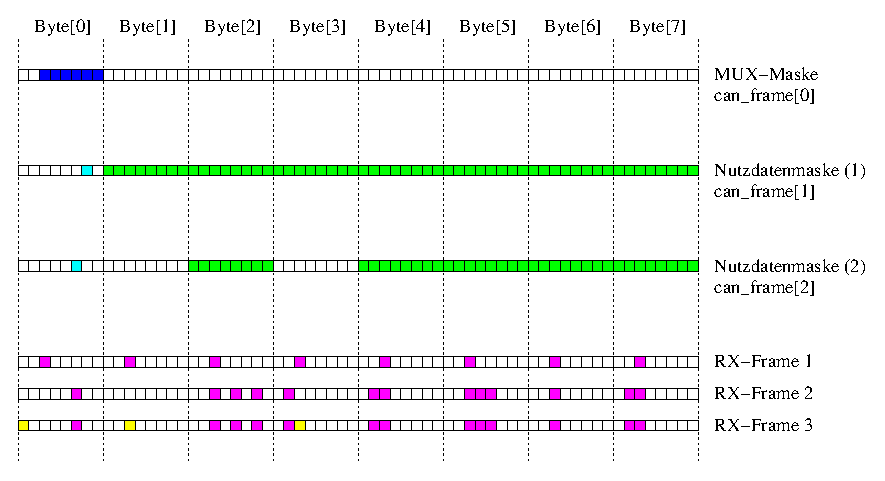
\psfig{file=bcm_mux_filter.eps}
\caption{Beispiel f�r die Anwendung des Multiplexfilters}
\label{figure:bcm_mux_filter}

\end{center}
\end{figure}

Eine �nderung einer Multiplex-Nachricht mit einem bestimmten
MUX-Identifier f�hrt zu einer Nachricht RX\_CHANGED
mit genau dem einen empfangenen CAN-Frame an den Prozess. D.h. der
Prozess muss anhand des MUX-Identifiers die vom \BCM\ empfangene
Nachricht bewerten.\\

Im gezeigten Beispiel (Abbildung \ref{figure:bcm_mux_filter}) ist die
MUX-Maske im Byte 0 auf \verb+0x5F+ 
gesetzt. Beim Empfang von RX-Frame 1 wird keine Nachricht an den
Anwender geschickt (MUX-Identifier ist nicht bekannt). Bei RX-Frame 2
gibt es eine Nachricht (MUX-Identifier bekannt und relevante Daten
haben sich - beim ersten Empfangsvorgang - ge�ndert). Beim Empfang von
RX-Frame 3 (�nderungen in den gelb markierten Bits) wird keine
Nachricht an den Anwender geschickt, weil sich
keine relevanten Daten f�r den eingetragenen MUX-Identifier ge�ndert haben.

\subsubsection{Nachrichtenfilterung (L�nge der Nutzdaten - DLC)}

Auf Anforderung kann der \BCM\ auch zus�tzlich eine Ver�nderung der in den
CAN-Nachrichten angegebenen Nutzdatenl�nge �berwachen. Dazu wird der
empfangene Data Length Code (DLC) mit dem zu diesem CAN-Frame
passenden, bereits empfangenen DLC verglichen. Ein Unterschied f�hrt
wie bei der Filterung der Nutzdaten zu einer Nachricht RX\_CHANGED an
den Prozess. Zum Aktivieren dieser Funktionalit�t muss in der
Komponente \verb+flags+ der Wert \verb+RX_CHECK_DLC+ gesetzt sein. 

\subsubsection{Filterung nach CAN-ID}

Im Gegensatz zu den oben beschriebenen Nachrichtenfiltern besteht auch
die M�glichkeit nur nach der angegebenen CAN-ID zu filtern. Dazu wird
in der Komponente \verb+flags+ der Wert \verb+RX_FILTER_ID+
gesetzt. Die Komponente \verb+nframes+ kann dabei Null sein und
so werden folglich auch keine Nutzdaten (\verb+can_frame+'s) an den
\BCM\ geschickt. Angeh�ngte Nutzdaten (d.h. \verb+nframes+ $>$ 0 und
entsprechende \verb+can_frame+'s) werden ignoriert. Werden
beim RX\_SETUP keine \verb+can_frames+ �bertrags, ist also
\verb+nframes+ = 0, wird im \BCM\ automatisch das Flag
\verb+RX_FILTER_ID+ gesetzt.\\

Hinweis: Die Filterung nach CAN-IDs sollte nur bei nicht zyklischen
CAN-Nachrichten genutzt werden.

\subsubsection{Automatisches Beantworten von RTR-Frames}
\label{rxrtrframe}

Grunds�tzlich k�nnen Remote-Transmission-Requests (RTR) mit dem \BCM\
ODER in einer Applikation im Userspace beantwortet werden. Im
Userspace w�rde eine Anwendung �ber den \BCM-Socket oder einen
RAW-Socket eine CAN-Nachricht empfangen, auf das gesetzte RTR-Bit
pr�fen und entsprechend eine Antwort senden. Das RX\_SETUP k�nnte in
diesem Fall beispielsweise so aussehen:

\begin{code}
    /* normal receiption of RTR-frames in Userspace */
    txmsg.msg_head.opcode  = RX_SETUP;
    txmsg.msg_head.can_id  = 0x123 | CAN_RTR_FLAG;
    txmsg.msg_head.flags   = RX_FILTER_ID;
    txmsg.msg_head.ival1.tv_sec = 0;
    txmsg.msg_head.ival1.tv_usec = 0;
    txmsg.msg_head.ival2.tv_sec = 0;
    txmsg.msg_head.ival2.tv_usec = 0;
    txmsg.msg_head.nframes = 0;

    if (write(s, &txmsg, sizeof(txmsg)) < 0)
      perror("write");
\end{code}

Diese Aufgabe kann auch der \BCM\ �bernehmen, indem man beim RX\_SETUP
statt eines Filters die auszusendende Nachricht angibt und das Flag
\verb+RX_RTR_FRAME+ setzt:

\begin{code}
    /* specify CAN-Frame to send as reply to a RTR-request */
    txmsg.msg_head.opcode  = RX_SETUP;
    txmsg.msg_head.can_id  = 0x123 | CAN_RTR_FLAG;
    txmsg.msg_head.flags   = RX_RTR_FRAME; /* | TX_CP_CAN_ID */;
    txmsg.msg_head.ival1.tv_sec  = 0; /* no timers in RTR-mode */
    txmsg.msg_head.ival1.tv_usec = 0;
    txmsg.msg_head.ival2.tv_sec  = 0;
    txmsg.msg_head.ival2.tv_usec = 0;
    txmsg.msg_head.nframes       = 1; /* exact 1 */

    /* the frame to send as reply ... */
    txmsg.frame.can_id    = 0x123; /* 'should' be the same */
    txmsg.frame.can_dlc   = 4;
    txmsg.frame.data[0]   = 0x12;
    txmsg.frame.data[1]   = 0x34;
    txmsg.frame.data[2]   = 0x56;
    txmsg.frame.data[3]   = 0x78;

    if (write(s, &txmsg, sizeof(txmsg)) < 0)
      perror("write");
\end{code}

Beim Empfang einer CAN-Nachricht mit der CAN-ID 0x123 und gesetztem
RTR-Bit wird das \verb+can_frame txmsg.frame+ ausgesendet. Bei
gesetztem Flag \verb+TX_CP_CAN_ID+ wird die Zeile mit
\verb+txmsg.frame.can_id+ obsolet. Der Wert \verb+txmsg.frame.can_id+
ist nicht beschr�nkt, 
d.h. der \BCM\ k�nnte auf ein RTR-Frame mit der CAN-ID 0x123 auch mit
einer CAN-Nachricht mit einer anderen CAN-ID (z.B. 0x42)
antworten. Achtung Denksportaufgabe: Bei gleicher CAN-ID und einem
gesetzten RTR-Flag im \verb+can_frame txmsg.frame+ erfolgt ein
Vollast-Test. Aus diesem Grunde wird bei Gleichheit von
\verb+txmsg.msg_head.can_id+ und \verb+txmsg.frame.can_id+ (z.B. bei
Anwendung der Option \verb+TX_CP_CAN_ID+) das RTR-Flag in
\verb+txmsg.frame.can_id+ beim RX\_SETUP automatisch gel�scht.

Die bei einem RTR-Frame auszusendende Nachricht kann durch ein erneutes
RX\_SETUP mit der identischen CAN-ID (mit gesetztem Flag
\verb+RX_RTR_FRAME+) jederzeit aktualisiert werden. Die
Nachrichtenl�nge f�r den Befehl RX\_SETUP mit gesetztem Flag
\verb+RX_RTR_FRAME+ ist \mbox{\tt \{[bcm\_msg\_head] [can\_frame]\} }
d.h. ein Nachrichtenkopf und genau ein CAN-Frame.\\

\subsection{RX\_DELETE}
\label{rxdelete}

Mit RX\_DELETE wird f�r eine bestimmte CAN-ID ein Empfangsauftrag
gel�scht. Die angegebene CAN-ID wird vom \BCM\ nicht mehr vom CAN-Bus
empfangen. 
Die Nachrichtenl�nge f�r den Befehl RX\_DELETE ist 
\mbox{\tt \{[bcm\_msg\_head]\} } d.h. ein Nachrichtenkopf.

\subsection{RX\_READ}
\label{rxread}

Mit RX\_READ kann der aktuelle Zustand des Filters f�r
CAN-Frames mit der angegebenen CAN-ID ausgelesen werden.  Der
Broadcast-Manager antwortet mit der Nachricht RX\_STATUS
an den Prozess. Diese
Antwort kann je nach L�nge der Daten beim zugeh�rigen RX\_SETUP
unterschiedlich lang sein.
Die Nachrichtenl�nge f�r den Befehl RX\_READ ist 
\mbox{\tt \{[bcm\_msg\_head]\} } d.h. ein Nachrichtenkopf.

\subsection{Weitere Anmerkungen zum Broadcast-Manager}
\label{bccomment}

\begin{quote}
\begin{itemize}
\item Die Nachrichten TX\_EXPIRED, RX\_TIMEOUT vom \BCM\ an den Prozess
enthalten keine Nutzdaten (\verb+nframes+ = 0)

\item Die Nachrichten TX\_STATUS, RX\_STATUS vom \BCM\ an den Prozess
enthalten genau so viele Nutzdaten, wie vom Prozess bei der
Einrichtung des Sende-/Empfangsauftrags mit TX\_SETUP bzw. RX\_SETUP
an den \BCM\ geschickt wurden.

\item Die Nachricht RX\_CHANGED vom \BCM\ an den Prozess
enth�lt genau das vom CAN empfangene, ge�nderte Nutzdaten-Frame
 (\verb+nframes+ = 1)

\item Beim �ndern von zu sendenden Multiplex-Nachrichten (TX\_SETUP)
m�ssen immer alle Nutzdaten-Frames �bertragen werden. Es wird generell
mit der Aussendung der ersten MUX-Nachricht begonnen.

\item Die Komponente \verb+can_id+ in der Struktur \verb+bcm_msg_head+
kann {\it sendeseitig} auch als 'Handle' betrachtet werden, weil bei der
Aussendung von CAN-Nachrichten die beim TX\_SETUP mit �bertragenen
\verb+can_frame+'s gesendet werden. Das Setzen jeder einzelnen
\verb+can_id+ in den \verb+can_frame+'s kann durch das Flag
\verb+TX_CP_CAN_ID+ vereinfacht werden.

\item Beim Auslesen der Sende-/Empfangsauftr�ge mit TX\_READ
bzw. RX\_READ k�nnen folgende Werte in den Antworten TX\_STATUS bzw.
RX\_STATUS von der urspr�nglich gesendeten Nachricht abweichen:
\begin{quote}
\begin{description}
\item[count] Entspricht dem aktuellen Wert
\item[SETTIMER] Wurde ausgef�hrt und damit konsumiert
\item[STARTTIMER] Wurde ausgef�hrt und damit konsumiert
\item[TX\_ANNOUNCE] Wurde ausgef�hrt und damit konsumiert
\end{description}
\end{quote}

\item Das Schlie�en des \BC-Sockets mit \man{close}{2} bzw. das
Terminieren des Anwenderprozesses l�scht alle Konfigurationseintr�ge
der zugeh�rigen \BC-Instanz. Zyklische Aussendungen dieser \BC-Instanz
werden folglich sofort beendet.

\end{itemize}
\end{quote}

\subsection{Testprogramme}

\begin{description}
\item[tst-bcm-single] f�hrt eine einzelne TX\_SEND-Operation aus.
\item[tst-bcm-cycle] Zyklisches Aussenden einer CAN-Botschaft mit
TX\_SETUP und beenden der zyklischen Aussendung mit
TX\_SETUP (ohne TX\_DELETE).
\item[tst-bcm-tx\_read] Funktionspr�fung der Debug-M�glichkeit mit TX\_READ.
\item[tst-bcm-rtr] Beispiel f�r die Anwendung des Flags \verb+RX_RTR_FRAME+.
\item[tst-bcm-filter] diverse Filtertests inklusive Multiplex-Filter.
\item[tst-bcm-throttle] Funktionspr�fung der Throttle-Funktionalit�t (Update-Bremse).
\item[can-sniffer] ist ein Programm zur Beobachtung dynamischer
Dateninhalte in zyklischen CAN-Nachrichten. �nderungen k�nnen in
hexadezimaler, bin�rer oder in ASCII-Darstellung farblich
hervorgehoben werden. Filter k�nnen zur Laufzeit ver�ndert und
gespeichert bzw. geladen werden.Wird \verb+can-sniffer+ ohne Parameter
aufgerufen, erscheint ein Hilfetext.
\end{description}


% $Id: procfs.tex,v 1.4 2006/02/08 14:38:21 hartko Exp $

\newpage
\section{\LL-Status im /proc-Filesystem}
\label{procfs}

Das \LLCF\ unterst�tzt das /proc-Filesystem und stellt dar�ber Statistiken
und Informationen �ber interne Strukturen und Stati in lesbarer Form zur
Verf�gung. Die Informationen k�nnen vom Benutzer beispielsweise mit\\

\verb+cat /proc/sys/net/can/stats+\\

abgefragt werden. Im Folgenden werden die einzelnen Eintr�ge erl�utert.

\subsection{Versionsinformation /proc/sys/net/can/version}

Die \LL-Versionsinformationen k�nnen f�r eine Anwendung z.B. durch das
�ffnen der Datei \verb+/proc/sys/net/can/version+ ausgelesen werden. Dazu werden
die ersten 6 Zeichen in einen Puffer kopiert und mit 
\verb+ llcf_version_code = strtoul(mybuffer, (char **)NULL, 16);+
in den LLCF\_VERSION\_CODE �berf�hrt. Der LLCF\_VERSION\_CODE wird
nach der Regel\\

\verb-LLCF_VERSION_CODE = (((MAJORVERSION) << 16) + ((MINORVERSION) << 8) + (PATCHLEVEL))-\\

berechnet.

\begin{code}
hartko@pplinux1:~> cat /proc/sys/net/can/version 
010000 [ Volkswagen AG - Low Level CAN Framework (LLCF) v1.0.0-rc1 ]
\end{code}

\subsection{Statistiken /proc/sys/net/can/stats}

�ber die angebotenen Statistiken kann man sich �ber das aktuelle
Datenaufkommen informieren und wie beispielsweise der Anteil der von
Applikationen ben�tigten (matched) CAN-Frames im Verh�ltnis aller vom CAN-Bus
empfangener CAN-Frames ist.\\

Die Informationen werden mit dem Start des \LL\ jede Sekunde aktualisiert.

\begin{code}
hartko@pplinux1:~> cat /proc/sys/net/can/stats 

      811 transmitted frames (TXF)
   319427 received frames (RXF)
    69504 matched frames (RXMF)

       21 % total match ratio (RXMR)
        0 frames/s total tx rate (TXR)
        0 frames/s total rx rate (RXR)

      100 % current match ratio (CRXMR)
        2 frames/s current tx rate (CTXR)
      166 frames/s current rx rate (CRXR)

      100 % max match ratio (MRXMR)
        2 frames/s max tx rate (MTXR)
      167 frames/s max rx rate (MRXR)

        6 current receive list entries (CRCV)
        6 maximum receive list entries (MRCV)

\end{code}
\subsection{Zur�cksetzen von Statistiken /proc/sys/net/can/reset\_stats}

Das Zur�cksetzen der statistischen Informationen kann durch interne
�berl�ufe von Z�hlern oder vom Benutzer selbst initiiert werden. �ber
das Zur�cksetzen der statistischen Informationen informiert eine
zus�tzliche Zeile (STR). An diesem Beispiel sind die Auswirkungen in
einem laufenden System bez�glich der obigen Ausgabe der Statistiken
gut zu erkennen.
\begin{code}
hartko@pplinux1:~> cat /proc/sys/net/can/reset_stats 
LLCF statistic reset #1 done.
hartko@pplinux1:~> cat /proc/sys/net/can/stats 

       31 transmitted frames (TXF)
     2585 received frames (RXF)
     2585 matched frames (RXMF)

      100 % total match ratio (RXMR)
        1 frames/s total tx rate (TXR)
      165 frames/s total rx rate (RXR)

      100 % current match ratio (CRXMR)
        2 frames/s current tx rate (CTXR)
      165 frames/s current rx rate (CRXR)

      100 % max match ratio (MRXMR)
        2 frames/s max tx rate (MTXR)
      167 frames/s max rx rate (MRXR)

        6 current receive list entries (CRCV)
        6 maximum receive list entries (MRCV)

        1 statistic resets (STR)


\end{code}

\subsection{Interne Empfangslisten des RX-Dispatchers}

\LL-Module k�nnen sich beim \LL-RX-Dispatcher f�r den Empfang von
einzelnen CAN-IDs (oder Bereichen von CAN-IDs) von bestimmten 
CAN-Netzwerk-Interfaces registrieren. Diese Registrierung f�hrt zu
einem Eintrag in einer zugeh�rigen Empfangsliste, bei der 
zu jeder registrierten CAN-ID eine Funktion mit einem Parameter
(z.B. eine modulspezifische Referenz wie 'userdata' oder 'sk')
aufgerufen wird, wenn das entsprechende CAN-Frame empfangen 
wurde. In der Spalte 'ident' tr�gt sich das
registrierende Protokoll-Modul namentlich ein. Zusammen mit der
Debug-Funktionalit�t (siehe Kapitel \ref{modparms}) kann man anhand
dieser Informationen die Funktionsweise des \LL\ einfach nachvollziehen.\\

Zur schnellen Verarbeitung empfangener CAN-Frames sind im
RX-Dispatcher des \LL\ verschiedenartige Empfangslisten (f�r jedes
CAN-Netzwerk-Interface) realisiert:

\begin{description}
\item[rcvlist\_all] In dieser Liste sind Registrierungen eingetragen,
die von einem CAN-Bus alle empfangenen CAN-Frames
ben�tigen. Typischerweise sind dieses die so genannten RAW-Sockets
ohne aktiven Filter (siehe Kapitel \ref{rawsocket}). 
\item[rcvlist\_fil] In dieser Liste sind Registrierungen eingetragen,
die nur einen �ber Bitmasken definierten Bereich von CAN-Frames
ben�tigen (z.B. 0x200 - 0x2FF).
\item[rcvlist\_inv] In dieser Liste sind Registrierungen eingetragen,
die einen �ber Bitmasken definierten Bereich von CAN-Frames ausblenden
wollen - also die Umkehrung von 'rcvlist\_fil'.
\item[rcvlist\_eff] In dieser Liste sind Registrierungen f�r einzelne
CAN-Frames im Extended Frame Format (29 Bit Identifier) eingetragen.
\item[rcvlist\_sff] In dieser Liste sind Registrierungen f�r einzelne
CAN-Frames im Standard Frame Format (11 Bit Identifier) eingetragen.
\end{description}

Durch das Aufteilen der Empfangslisten, wird der Aufwand zum Suchen
und Vergleichen des empfangenen CAN-Frames mit den registrierten
Empfangsfiltern minimiert.\\

So wurde z.B. die Liste 'rcvlist\_sff' als Array mit 2048 Eintr�gen (11 Bit
CAN-ID) mit einer einfach verketteten Liste f�r die jeweiligen CAN-IDs
realisiert. Auf eine �berpr�fung von Filtern und Inhalten kann hier
beim Empfang einer passenden Nachricht verzichtet werden.\\

Derzeit
wird die Funktionalit�t der Extended CAN-Frames in aktuellen Projekten
nicht genutzt, weshalb die Registrierungen f�r einzelne EFF-Frames in
eine einfach verkettete Liste eingetragen werden. Bei intensiverer
Nutzung der Extended CAN-Frames sollte man als 'rcvlist\_eff' eine
Hash-Tabelle (analog zur 'rcvlist\_sff') im \LL\ realisieren, um eine
effiziente Verarbeitung zu gew�hrleisten.\\ 

M�chte man alle Empfangslisten auf einmal ansehen, kann man zur
Vereinfachung folgendes eingeben:

\begin{code}
hartko@pplinux1:~> cat /proc/sys/net/can/rcvlist_*

receive list 'rx_all':
  device   can_id   can_mask  function  userdata   matches  ident
   can1      000    00000000  f8c995ac  f0e59280     42726  raw
  device   can_id   can_mask  function  userdata   matches  ident
   can0      000    00000000  f8c995ac  f0e59800     55240  raw


receive list 'rx_eff':
  (can1: no entry)
  (can0: no entry)


receive list 'rx_fil':
  device   can_id   can_mask  function  userdata   matches  ident
   can1      200    00000700  f8c995ac  f0e5b380         0  raw
  (can0: no entry)


receive list 'rx_inv':
  (can1: no entry)
  (can0: no entry)


receive list 'rx_sff':
  (can1: no entry)
  device   can_id   can_mask  function  userdata   matches  ident
   can0      123    000007ff  f8c86bec  e2e14380        29  bcm
   can0      456    000007ff  f8c86bec  ea954880         0  bcm
   can0      789    000007ff  f8c86bec  e30e6200       130  bcm
   can0      3FF    000007ff  f8c86bec  deaf2580        14  bcm
   can0      740    000007ff  f8c93680  e48322c4       178  tp20

\end{code}

Es geht nat�rlich auch so:

\begin{code}
hartko@pplinux1:~> cat /proc/sys/net/can/rcvlist_sff

receive list 'rx_sff':
  (can1: no entry)
  device   can_id   can_mask  function  userdata   matches  ident
   can0      123    000007ff  f8c86bec  e2e14380        29  bcm
   can0      456    000007ff  f8c86bec  ea954880         0  bcm
   can0      789    000007ff  f8c86bec  e30e6200       130  bcm
   can0      3FF    000007ff  f8c86bec  deaf2580        14  bcm
   can0      740    000007ff  f8c93680  e48322c4       178  tp20

\end{code}

\newpage
\subsection{CAN Network-Devices im Verzeichnis /proc/net/drivers}

In dieses Verzeichnis sollen sich CAN-Netzwerk-Treiber mit ihren
Proc-Filesystem-Eintr�gen registrieren. Derzeit ist dieses nur f�r den
mitgelieferten SJA1000-Treiber auf \verb+src/drivers/sja1000+
realisiert, dessen Ausgaben kurz beschrieben werden.\\

Im Beispiel wird der SJA1000-Netzwerk-Treiber auf dem iGate (Jaybrain
GW2) gezeigt. Beim ISA-Treiber (sja1000-isa) sind die ausgelesenen
Informationen analog.
 
\subsubsection{Treiberstatus /proc/net/drivers/sja1000-xxx}

Hier wird der Zustand der CAN-Controller und des jeweils zugeh�rigen
CAN-Busses angezeigt (siehe dazu die Dokumentation zum Philips
SJA1000).

\begin{code}
hartko@pplinux1:~> cat /proc/net/drivers/sja1000-gw2
CAN bus device statistics:
       errwarn  overrun   wakeup   buserr   errpass  arbitr   restarts clock        baud
can0:        0        0        0        0        0        0        0   20000000      500
can0: bus status: OK, RXERR: 0, TXERR: 0
can1:        0        0        0        0        0        0        0   20000000      100
can1: bus status: OK, RXERR: 0, TXERR: 0
can2:        0        0        0        0        0        0        0   20000000      100
can2: bus status: OK, RXERR: 0, TXERR: 0
can3:        0        0        0        0        0        0        0   20000000      500
can3: bus status: OK, RXERR: 0, TXERR: 0
\end{code}

\subsubsection{Registeranzeige /proc/net/drivers/sja1000-xxx\_regs}

Hier werden die 32 Register der SJA1000-CAN-Controller angezeigt
(siehe dazu die Dokumentation zum Philips SJA1000).

\begin{code}
hartko@pplinux1:~> cat /proc/net/drivers/sja1000-gw2_regs 
SJA1000 registers:
can0 SJA1000 registers:
00: 02 00 0c 00 05 00 40 4d 1a 1a 00 00 00 60 00 00
10: 65 ef d3 5f a2 08 01 05 fa ff 0e 7f 0c 00 00 cf
can1 SJA1000 registers:
00: 02 00 0c 00 05 00 43 ff 1a 1a 00 00 00 60 00 00
10: 61 ff de 3d 80 00 10 45 d7 ef fb 4a 06 00 00 cf
can2 SJA1000 registers:
00: 02 00 0c 00 05 00 43 ff 1a 1a 00 00 00 60 00 00
10: 61 fb ee 87 a0 4a 80 10 76 ff da bd 00 00 00 cf
can3 SJA1000 registers:
00: 02 00 0c 00 05 00 40 4d 1a 1a 00 00 00 60 00 00
10: 61 ef 7f ff 21 1c 42 08 32 df 57 6f a1 00 00 cf
\end{code}

\subsubsection{Zur�cksetzen des Treibers /proc/net/drivers/sja1000-xxx\_reset}

Das Lesen dieses Eintrages f�hrt einen Reset der SJA1000-CAN-Controller
durch. Wie man im Beispiel sieht, ist die Anzahl der 'restarts' danach
um 1 erh�ht.

\begin{code}
hartko@pplinux1:~> cat /proc/net/drivers/sja1000-gw2_reset 
resetting can0 can1 can2 can3 done
hartko@pplinux1:~> cat /proc/net/drivers/sja1000-gw2
CAN bus device statistics:
       errwarn  overrun   wakeup   buserr   errpass  arbitr   restarts clock        baud
can0:        0        0        0        0        0        0        1   20000000      500
can0: bus status: OK, RXERR: 0, TXERR: 0
can1:        0        0        0        0        0        0        1   20000000      100
can1: bus status: OK, RXERR: 0, TXERR: 0
can2:        0        0        0        0        0        0        1   20000000      100
can2: bus status: OK, RXERR: 0, TXERR: 0
can3:        0        0        0        0        0        0        1   20000000      500
can3: bus status: OK, RXERR: 0, TXERR: 0
\end{code}

\subsubsection{Testprogramme}

\begin{description}
\item[tst-proc] �ffnet bis zu 800 RAW-Sockets, um einen �berlauf bei
der Ausgabe von \verb+/proc/net/can/rcvlist_all+ zu provozieren.
\end{description}


% $Id: hardware.tex,v 1.3 2006/02/20 07:35:44 hartko Exp $

\newpage
\section{Unterst�tzte CAN-Hardware}
\label{hardware}

Bisherige Realisierungen von CAN-Treibern unter
Linux und auch anderen Betriebssystemen sind nach dem
Zeichen-Treibermodell (dem so genannten Character-Device) ausgef�hrt.\\

Im Unterschied dazu setzt das \LLCF\ auf
CAN-Treiber nach dem Netzwerk-Treibermodell auf (so genannte
Network-Devices), die es erm�glichen, dass mehrere Anwendungen
gleichzeitig auf einem CAN-Bus arbeiten k�nnen.\\

Wenngleich ein Treiber nach dem Netzwerk-Treibermodell einfacher zu
realisieren ist, sind die bei einer kommerziellen CAN-Hardware
beigelegten Treiber f�r das \LL\ so nicht einsetzbar. Ist der
Quellcode des beigelegten Treibers verf�gbar, kann man diesen
allerdings so modifizieren, dass er sich nicht als Character-Device
sondern als Network-Device im Linux-Kernel registriert und entsprechend
andere Schnittstellen des Kernel bedient.\\

Der unter \verb+src/drivers/sja1000+ realisierte
Philips-SJA1000-Treiber ist eine 
komplette Neuentwicklung und kann als Beispiel f�r einen
CAN-Netzwerktreiber genommen werden. Derzeit unterst�tzt das \LL\
ausschlie�lich passive CAN-Karten, weil dieses f�r den Linux-Kernel im
Gegensatz zu anderen Betriebssystemen problemlos m�glich ist. Ein
modifizierter Treiber f�r eine aktive PCMCIA-Karte ist in Arbeit.\\

Derzeit werden folgende CAN-Hardware-Komponenten unterst�tzt:
\subsection{PC104 / ISA / plain access}

In diesen Karten liegen die SJA1000-Controller linear im Adressraum.\\
Z.B. http://www.peak-system.com/db/de/pcanpc104.html\\

M�gliche Treiber:
\begin{itemize}
\item \LL-SJA1000-Treiber in \verb+src/drivers/sja1000+ (empfohlen)
\item Modifizierter Linux-Treiber v2.15 von PEAK-System (auf Anfrage)
\end{itemize}

\subsection{PCI}

In diesen Karten liegen die SJA1000-Controller linear im
PCI-Adressraum.\\
Z.B. http://www.peak-system.com/db/de/pcanpci.html\\

M�gliche Treiber:
\begin{itemize}
\item Modifizierter Linux-Treiber v2.15 von PEAK-System (auf Anfrage)
\end{itemize}

\subsection{Parallelport}

Ben�tigt Linux-Parport-Unterst�tzung.\\
Z.B. http://www.peak-system.com/db/de/pcandongle.html\\

M�gliche Treiber:
\begin{itemize}
\item Modifizierter Linux-Treiber v2.15 von PEAK-System (auf Anfrage)
\end{itemize}

\subsection{USB}

USB-CAN-Adapter.\\
http://www.peak-system.com/db/de/pcanusb.html\\

M�gliche Treiber:
\begin{itemize}
\item Modifizierter Linux-Treiber v2.15 von PEAK-System
\end{itemize}

\subsection{PCMCIA}

Passive PCMCIA-Karte mit zwei SJA1000-Controllern.\\
http://www.ems-wuensche.com/catalog/english/datasheet/htm/cpccard\_e.htm\\

M�gliche Treiber:
\begin{itemize}
\item Modifizierter Linux-Treiber cdkl-1.12 von EMS W�nsche (auf Anfrage)
\end{itemize}

Aktive PCMCIA-Karte mit zwei SJA1000-Controllern.\\
http://www.kvaser.com/prod/hardware/lapcan\_i.htm\\
http://www.kvaser.com/prod/hardware/lapcan\_ii.htm\\

M�gliche Treiber (in Arbeit!):
\begin{itemize}
\item Modifizierter Linux-Treiber v4.1beta von Kvaser
\end{itemize}


\subsection{Virtual CAN Bus (vcan)}

Der virtuelle CAN-Bus-Treiber realisiert ein logisches
CAN-Network-Device, �ber das Anwendungen auf einem System ohne real
vorhandene CAN-Hardware kommunizieren k�nnen. Die Idee entspricht
einem Loopback-Device, wobei die Loopback-Funktionalit�t (siehe
Kapitel \ref{intro}) bereits im \LL-Rahmen realisiert ist. Der
vcan-Treiber ist Bestandteil des \LLCF.

\newpage

\section{Ansprechpartner}

Dieses Dokument sollte zusammen mit den Test-Programmen in
\verb+src/test+ einen umfassenden Einstieg in das \LLCF\
erm�glichen.\\

F�r R�ckfragen, Fehlermeldungen und Anregungen sind die Autoren
dennoch immer offen und dankbar. Deshalb hat die Konzernforschung
der Volkswagen AG eine besondere EMail-Adresse eingerichtet, auf der
die Autoren erreichbar sind:\\

{\Large \tt contact email: llcf@volkswagen.de}\\

Postadresse:\\
Volkswagen AG\\
Oliver Hartkopp\\
Brieffach 1776\\
D-38426 Wolfsburg\\

Oliver Hartkopp $<$oliver.hartkopp@volkswagen.de$>$\\
Dr. Urs Th�rmann $<$urs.thuermann@volkswagen.de$>$

\end{document}
